\chapter{Instalación do sistema Caronte}

Neste apéndice detallaranse as principais fases para a instalación e posta a punto do noso sistema Caronte.
En primeiro lugar, indicaranse os requisitos do sistema. A continuación, os pasos para a súa instalación e despregue, tanto do servidor como da aplicación Android.
Por último, remataremos co manual do usuario e unha guía rápida de funcionamento para os tres roles que se distinguen no sistema: administrador, xestor de contido e usuario final.

\section{Requisitos}
A continuación expóñense os requisitos necesarios para a instalación do noso sistema, tanto os servizos web coa base de datos, coma a aplicación móbil.

\subsection{Servidor Caronte}
A continuación enuméranse os requisitos necesarios para o funcionamento do noso servidor:

\begin{itemize}
	\item Servidor con alta dispoñibilidade.
	\item Contedor de servlets Java para despregar os servizos web.
	\item Base de datos.
	\item Bo largo de banda.
	\item Disco duro con 20 MB libres. Serían necesarios máis se se queren engadir imaxes.
\end{itemize}

\subsection{Aplicación Android: Caronte}
Para poder instalar e utilizar a aplicación, requírese un dispositivo móbil que cumpra unha serie de requisitos software, pero sobre todo hardware. A lista de necesidades pódese ver a continuación:

\begin{itemize}
	\item Sistema operativo Android superior ou igual á versión 4.4 (Kit Kat).
	\item Sensor GPS.
	\item Conexión Wi-Fi.
	\item Conexión datos.
	\item Bluetooth (recomendado).
	\item 1,5 GB de memoria RAM para un uso .
	\item 7 MB libres de espazo no dispositivo. Máis se se desexan visualizar imaxes de puntos de interese.
\end{itemize}

\section{Instalación}
A continuación describiremos os pasos principais requiridos para a instalación tanto do servidor Caronte coma da aplicación Android.

\subsection{Servidor Caronte}
Para o despregue do noso servidor, tivemos que crear unha conta en Amazon Web Services mais valería calquera outra plataforma de computación na nube na cal aloxar o noso servidor.

Entre as múltiples opcións dentro da conta de AWS, permítese arrincar imaxes de distribucións Linux nas cales poder instalar todo o software que precisemos. Grazas a isto púidose instalar o contedor de servlets Java Apache Tomcat na súa versión 8. Outra das opcións incluídas no servizo é a de arrincar unha base de datos. A opción escollida foi PostgreSQL.

Para o almacenamento de imaxes foi preciso crear unha carpeta especial sobre a cal o Tomcat tivese permisos de escritura para poder deixar as imaxes nun punto concreto.

\subsection{Aplicación Android: Caronte}
A instalación da aplicación pode levarse a cabo a través da tenda oficial de Google: Google Play. Non obstante, tamén se pode proceder á instalación manual do arquivo APK se se habilita a instalación de aplicacións con orixe descoñecida nos axustes de seguridade do teléfono.

Non hai ningún tipo de necesidade a maiores no momento da instalación, xa que a petición de permisos necesarios para o funcionamento da aplicación solicítanse dinamicamente na súa execución.

\section{Manual de usuario do servidor Caronte}
A continuación exporemos os pasos a realizar para a configuración do noso servidor que nos permitirá a execución dos nosos servizos.

\subsection{Creación da imaxe en AWS}
O primeiro paso para poñer en funcionamento o sistema foi crear unha conta de usuario dentro de Amazon Web Services. Se non se require unha gran potencia de cálculo, disponse dun período de proba de 1 ano durante o cal é posíbel utilizar os servizos sen pagar sempre e cando non se supere un límite que en condicións normais non se pasaría. O formulario de creación de conta pódese ver na figura~\ref{fig:AWSCrear}.

\begin{figure}[h]
	\begin{center}
		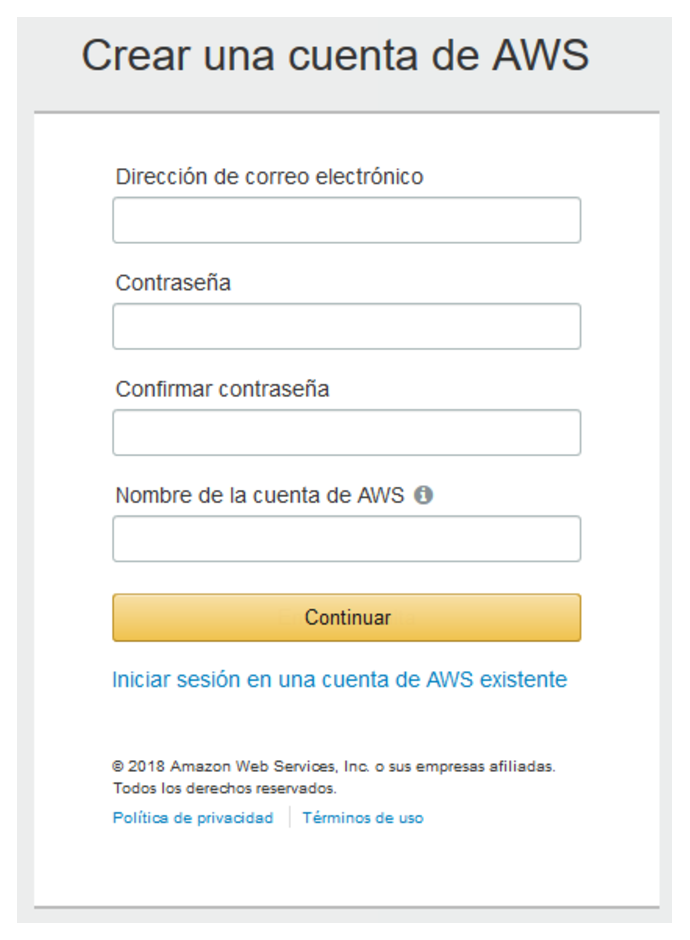
\includegraphics[width=0.5\textwidth]{figures/capturas/AWSCrear}
		\caption{Pantalla de creación de conta en Amazon Web Services.}
		\label{fig:AWSCrear}
	\end{center}
\end{figure}


Unha vez se crea a conta, tense acceso a múltiples servizos dentro da consola de xestión. O segundo paso sería crear unha imaxe dunha distribución Linux onde despois poder despregar o noso servizo web, como se pode ver na figura~\ref{fig:AWSImaxes}. Hai unha gran cantidade de opcións para escoller, non unicamente distribucións Linux, senón tamén imaxes de sistemas Windows. 

\begin{figure}[h]
	\begin{center}
		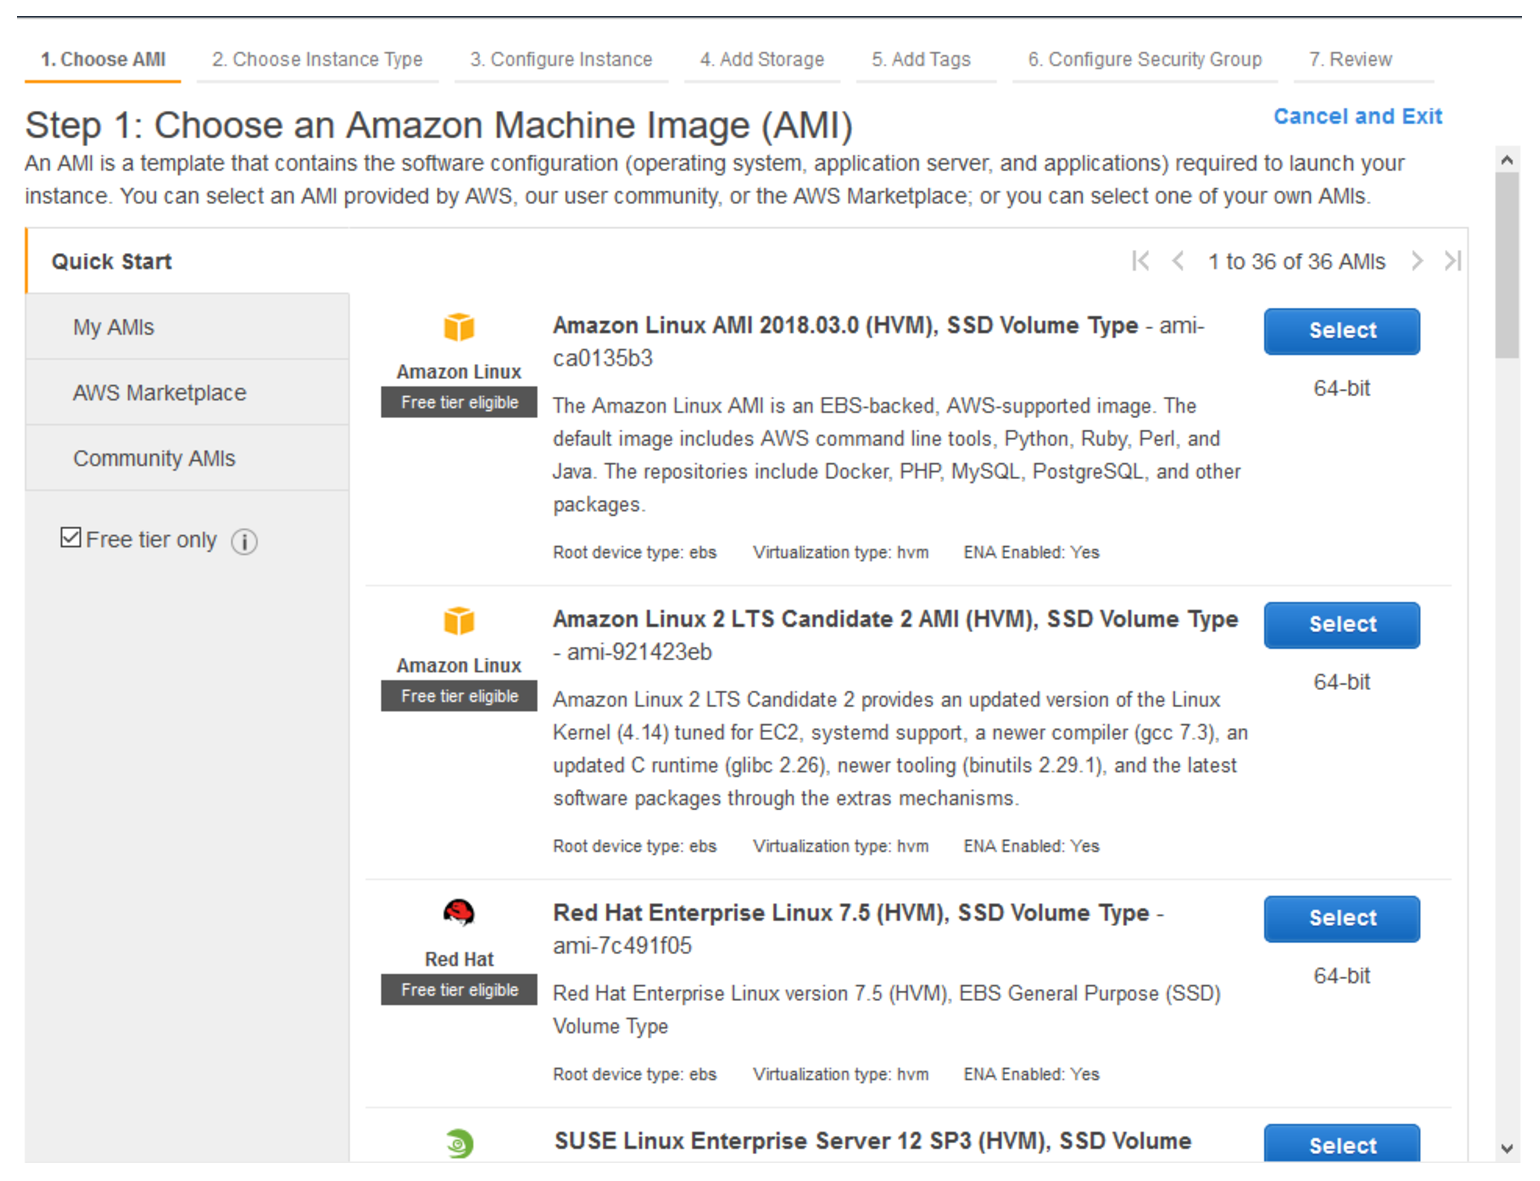
\includegraphics[width=0.9\textwidth]{figures/capturas/AWSImaxes}
		\caption{Pantalla para a selección de imaxe en Amazon Web Services.}
		\label{fig:AWSImaxes}
	\end{center}
\end{figure}

\subsection{Base de datos}
Outro paso imprescindíbel para iniciar o noso sistema é a base de datos. Amazon Web Services dispón dunha gran variedade de xestores de bases de datos entre os cales elixir, como se pode ver na imaxe~\ref{fig:AWSBD}. No noso caso, escolleuse un motor PostgreSQL.

\begin{figure}[h]
	\begin{center}
		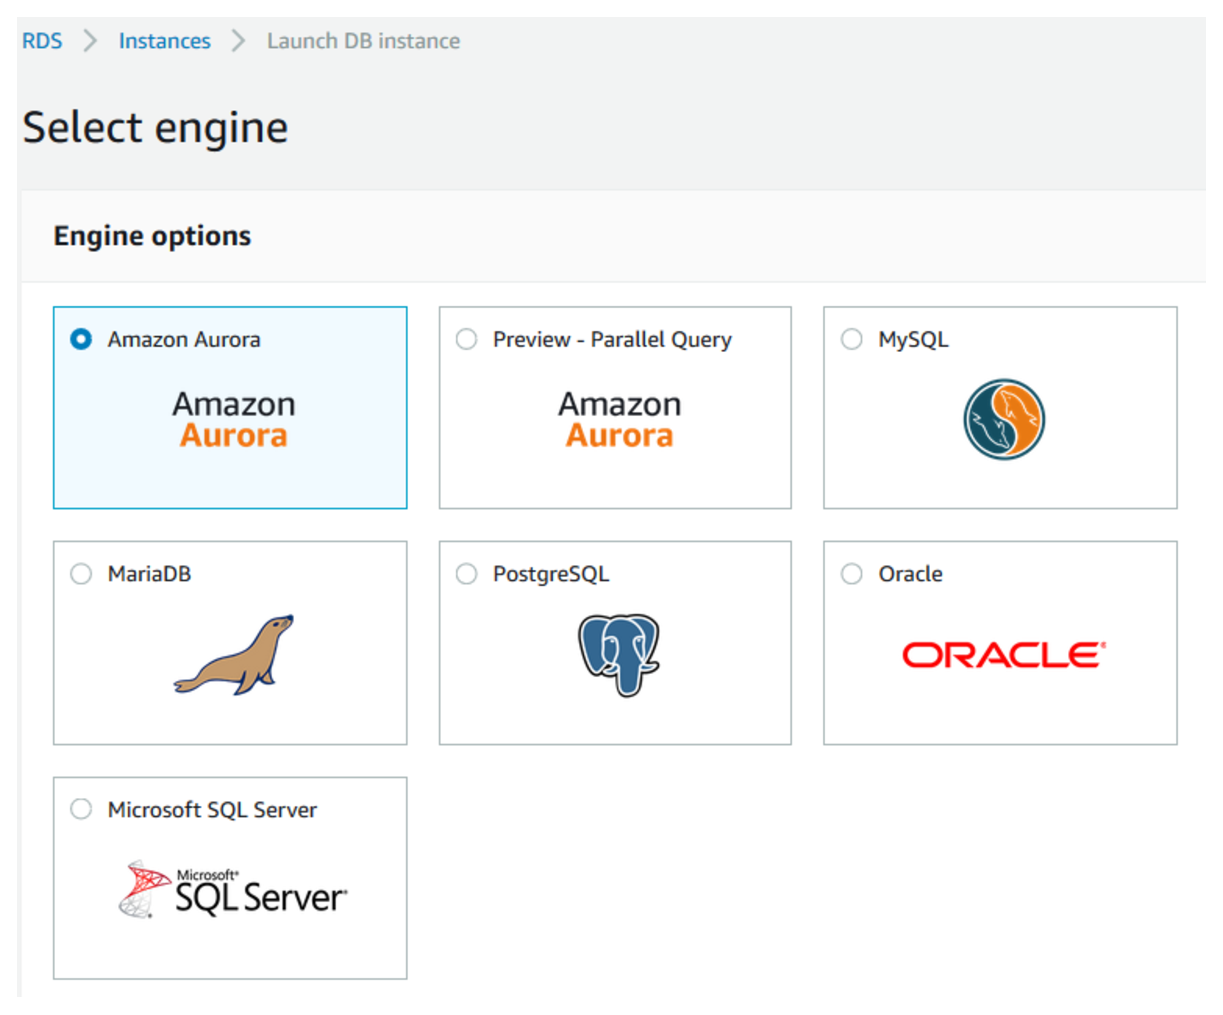
\includegraphics[width=0.75\textwidth]{figures/capturas/AWSBD}
		\caption{Pantalla para a selección da base de datos en Amazon Web Services.}
		\label{fig:AWSBD}
	\end{center}
\end{figure}

\subsection{Conexión coa imaxe}
Cando se teña instalada a imaxe, debemos configurar a conexión con ela. Optouse por realizar estas conexións dende o PuTTY, un cliente telnet para Windows. A configuración da conexión coa nosa instancia de Linux está perfectamente detallada no manual de Amazon Web Services \cite{manualAWSPutty}, mais indicaremos os puntos principais para levar a cabo unha conexión exitosa:


\begin{figure}[h]
	\begin{center}
		\includegraphics[width=0.6\textwidth]{figures/capturas/putty}
		\caption{Configuración da conexión con PuTTY.}
		\label{fig:putty}
	\end{center}
\end{figure}

\begin{itemize}
	\item Instalar PuTTY.
	\item Obter a información sobre a imaxe na consola de AWS: identificador e nome DNS público.
	\item Identificar o nome de usuario co que se lanzou a instancia.
	\item Permitir na consola de AWS a conexión SSH (porto 22) dende o noso equipo.
	\item Localizar a chave privada do ficheiro .pem especificado ao lanzar a imaxe.
	\item Converter a chave privada con PuTTYgen.
	\item Iniciar PuTTY.
	\item Configurar acceso á imaxe indicando como hostname nome\_usuario@nome\_dns\_publico e porto 22.
	\item No panel de Category -> Connection -> Auth, seleccionar a chave privada xerada por PuTTYgen.
	\item Gardar a configuración.
	\item Lanzar a conexión.
\end{itemize}

\subsection{Instalación contedor de servlets}
Dende a nosa imaxe Linux poderemos instalar todo tipo de paquetes mediante o comando \emph{apt-get install}. Para a instalación do contedor de servlets, optouse polo Apache Tomcat na súa versión 8. Para iniciar a instalación, execútase a seguinte sentencia:

\begin{lstlisting}
sudo apt-get install tomcat8 tomcat8-docs tomcat8-admin
\end{lstlisting}

Unha vez rematada a instalación, debemos modificar o ficheiro tomcat-users.xml para restrinxir o acceso ao usuario co rol que se indica na figura~\ref{fig:tomcatUsers}.

\begin{figure}[h]
	\begin{center}
		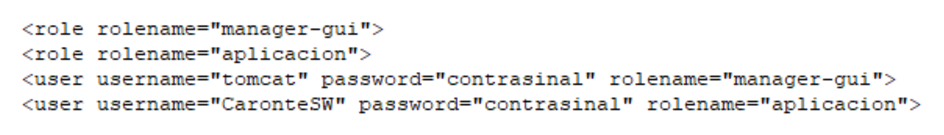
\includegraphics[width=0.8\textwidth]{figures/capturas/tomcatUsers}
		\caption{Configuración do ficheiro tomcat-users.xml.}
		\label{fig:tomcatUsers}
	\end{center}
\end{figure}

Por último, reiniciamos o servidor:

\begin{lstlisting}
sudo systemctl restart tomcat8
\end{lstlisting}

\subsection{Despregue dos servizos}
Dende á dirección direccionImaxe:8080/manager/html pódese acceder á páxina de xestión de aplicación do Tomcat grazas ao usuario con rol manager-gui e ao contrasinal indicados en tomcat-users. Nela pódense despregar, parar ou replegar aplicacións web. Dende está ventá será dende onde subamos a nosa aplicación empaquetada en formato \emph{.war}, como se ve na imaxe~\ref{fig:tomcatXestor}. Unha vez despregada poderemos acceder aos nosos servizos.

\begin{figure}[h]
	\begin{center}
		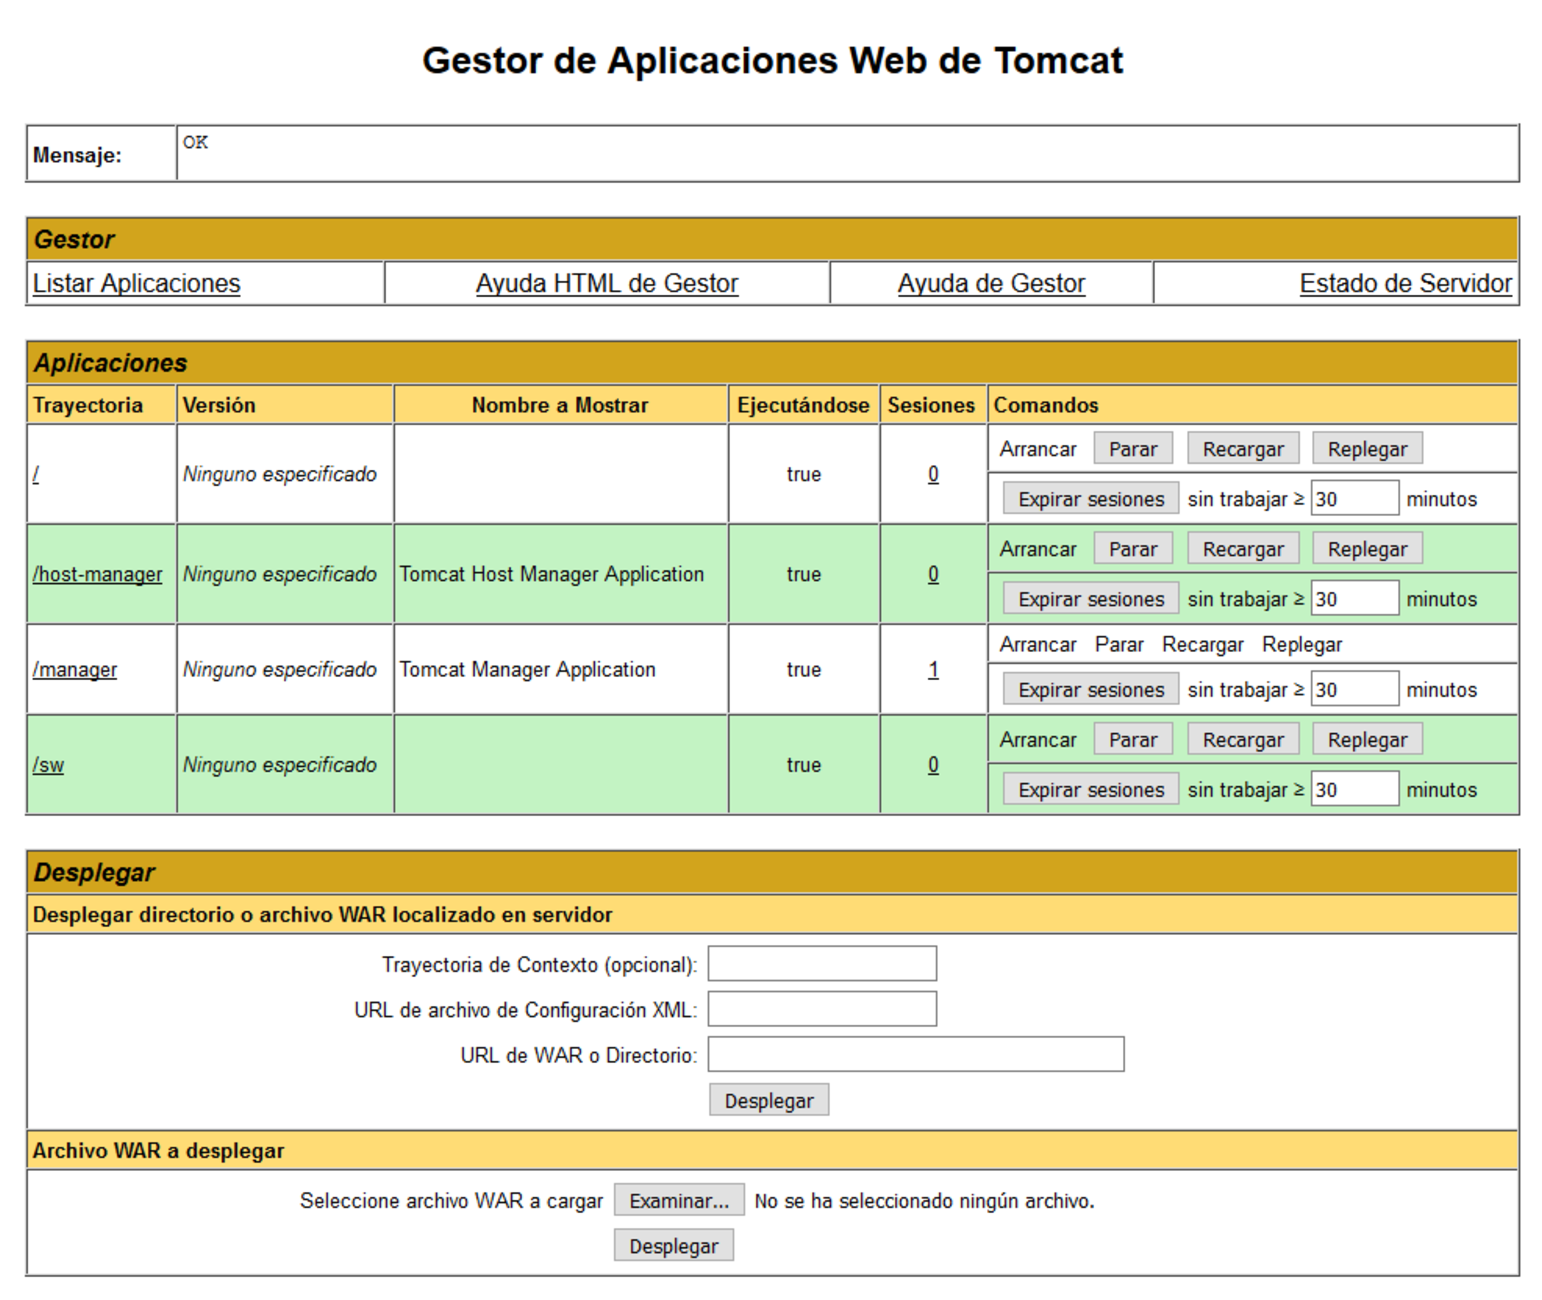
\includegraphics[width=0.9\textwidth]{figures/capturas/tomcatXestor}
		\caption{Páxina de xestión das aplicacións do Tomcat.}
		\label{fig:tomcatXestor}
	\end{center}
\end{figure}


\subsection{Mantemento}
O administrador do sistema terá que realizar tarefas de mantemento que consistirán, basicamente, en dar de alta novos edificios en base de datos, así coma asignar contas de Situm a usuarios concretos e proporcionar o rol de xestor de contido a certos usuarios. Estas accións realízanse dende un xestor de base de datos, como pode ser o SQuirreL. Para coñecer os identificadores dos usuarios, os edificios e as contas de Situm, débese acceder ás súas táboas.

Consulta e inserción de edificios:
\begin{lstlisting}
SELECT * FROM MUSEO.EDIFICIO;

INSERT INTO MUSEO.EDIFICIO (ID_EDIFICIO, ID_EDIFICIO_EXTERNO, NOME, DESCRICION) VALUES (4, 3000, 'Museo do Prado', 'Museo do Prado');
\end{lstlisting}

Consulta de usuarios e contas de Situm:
\begin{lstlisting}
SELECT * FROM MUSEO.USUARIO;

SELECT * FROM MUSEO.CONTA_SITUM;
\end{lstlisting}

Asociación de conta Situm a usuario concreto:
\begin{lstlisting}
INSERT INTO MUSEO.CONTA_SITUM_USUARIO (ID_CONTA_SITUM, ID_USUARIO) VALUES (1, 5);
\end{lstlisting}

Asignación do rol xestor de contido a un usuario concreto sobre un edificio:
\begin{lstlisting}
INSERT INTO MUSEO.USUARIO_EDIFICIO (ID_USUARIO, ID_EDIFICIO, ADMINISTRADOR) VALUES (5, 4, 1);
\end{lstlisting}


\section{Manual de usuario da aplicación Caronte}
Nesta sección explícase o funcionamento da aplicación para os usuarios sen rol de xestor de contido (que se verá no seguinte punto). Utilizaranse capturas de pantalla para unha mellor comprensión.

\begin{figure}[h]
	\begin{center}
		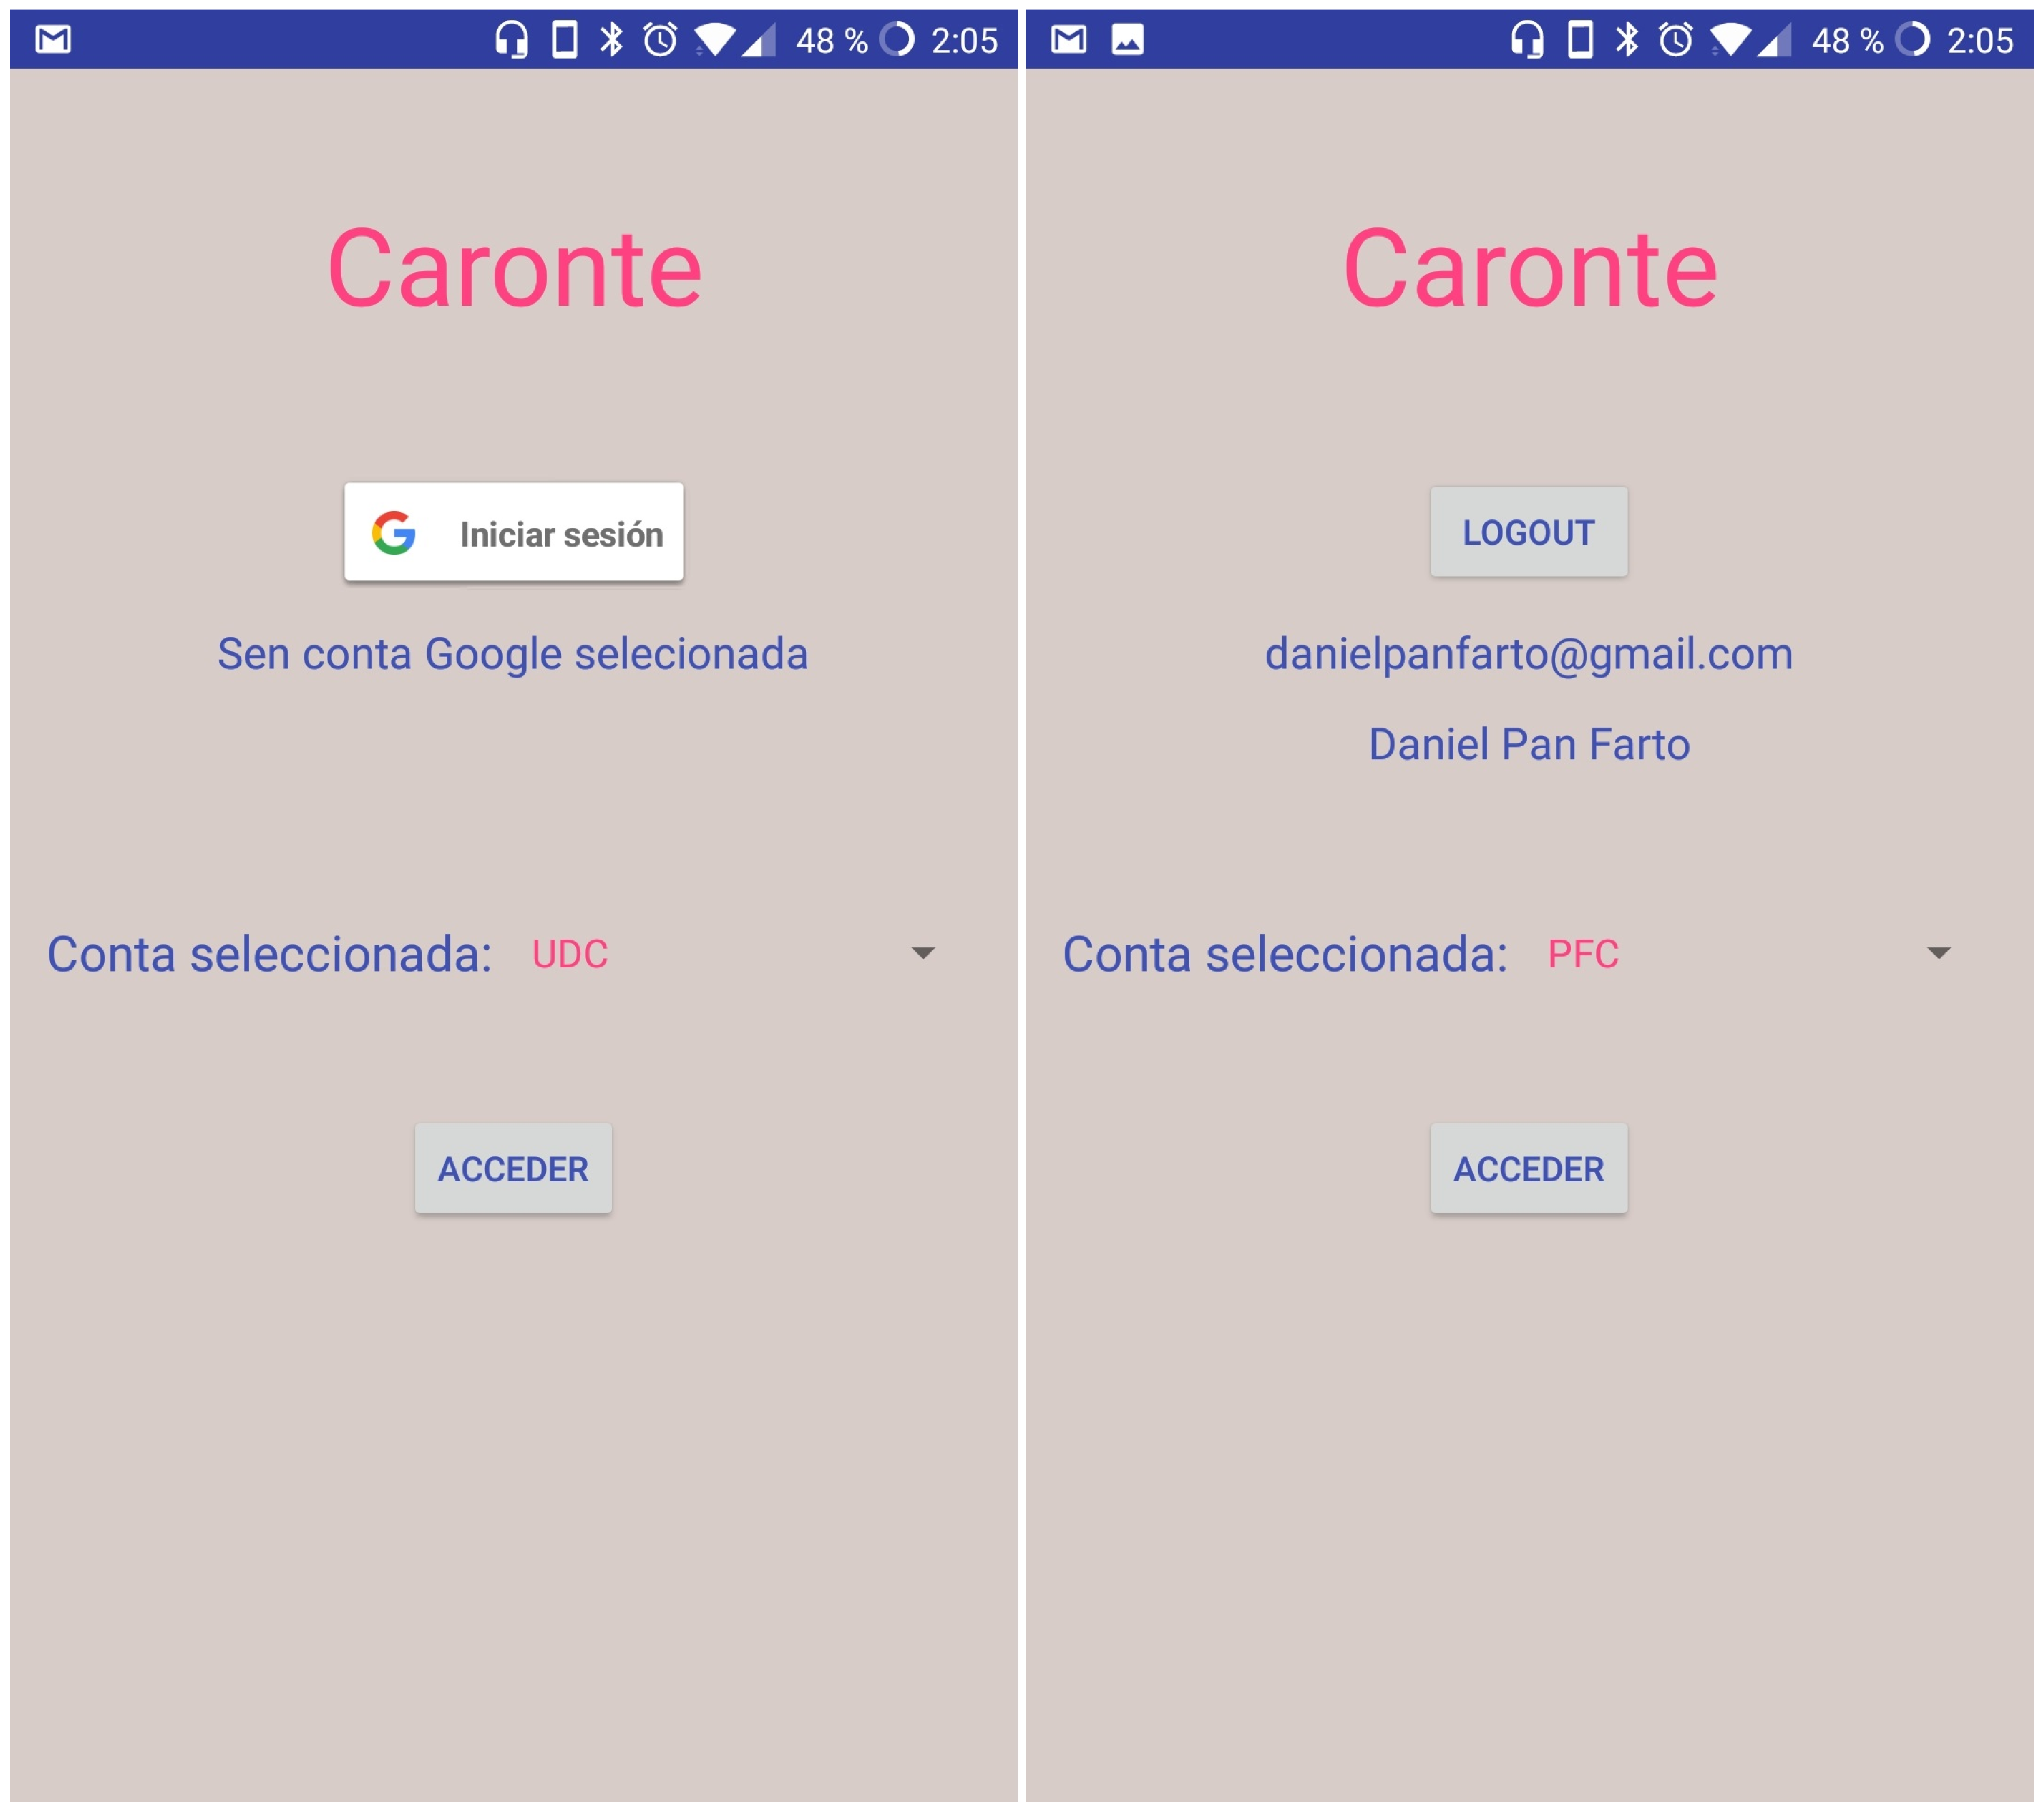
\includegraphics[width=0.5\textwidth]{figures/android/capturaInicio}
		\caption{Pantalla de inicio previa ao login (esquerda) e posterior (dereita).}
		\label{fig:capturaInicio}
	\end{center}
\end{figure}

\subsection{Inicio}
É a primeira pantalla que verá un usuario que abra a aplicación. É unha vista moi sinxela que só se compón de dous botóns (autenticación con Google e acceso ao mapa) e un spinner para seleccionar a conta de Situm coa que conectarnos (ver primeira captura da figura~\ref{fig:capturaInicio}). O botón superior permite autenticarse cunha conta de Google, o que permitirá acceder a contas de Situm que teñamos asociadas en base de datos ao noso usuario, a maiores das que están marcadas como públicas. Cando un usuario está autenticado, aparece un novo botón que permite facer logout (ver segunda captura da figura~\ref{fig:capturaInicio}). Pulsando sobre o botón ACCEDER pasaremos á seguinte pantalla, que é a principal, a do mapa.

\begin{figure}[h]
	\begin{center}
		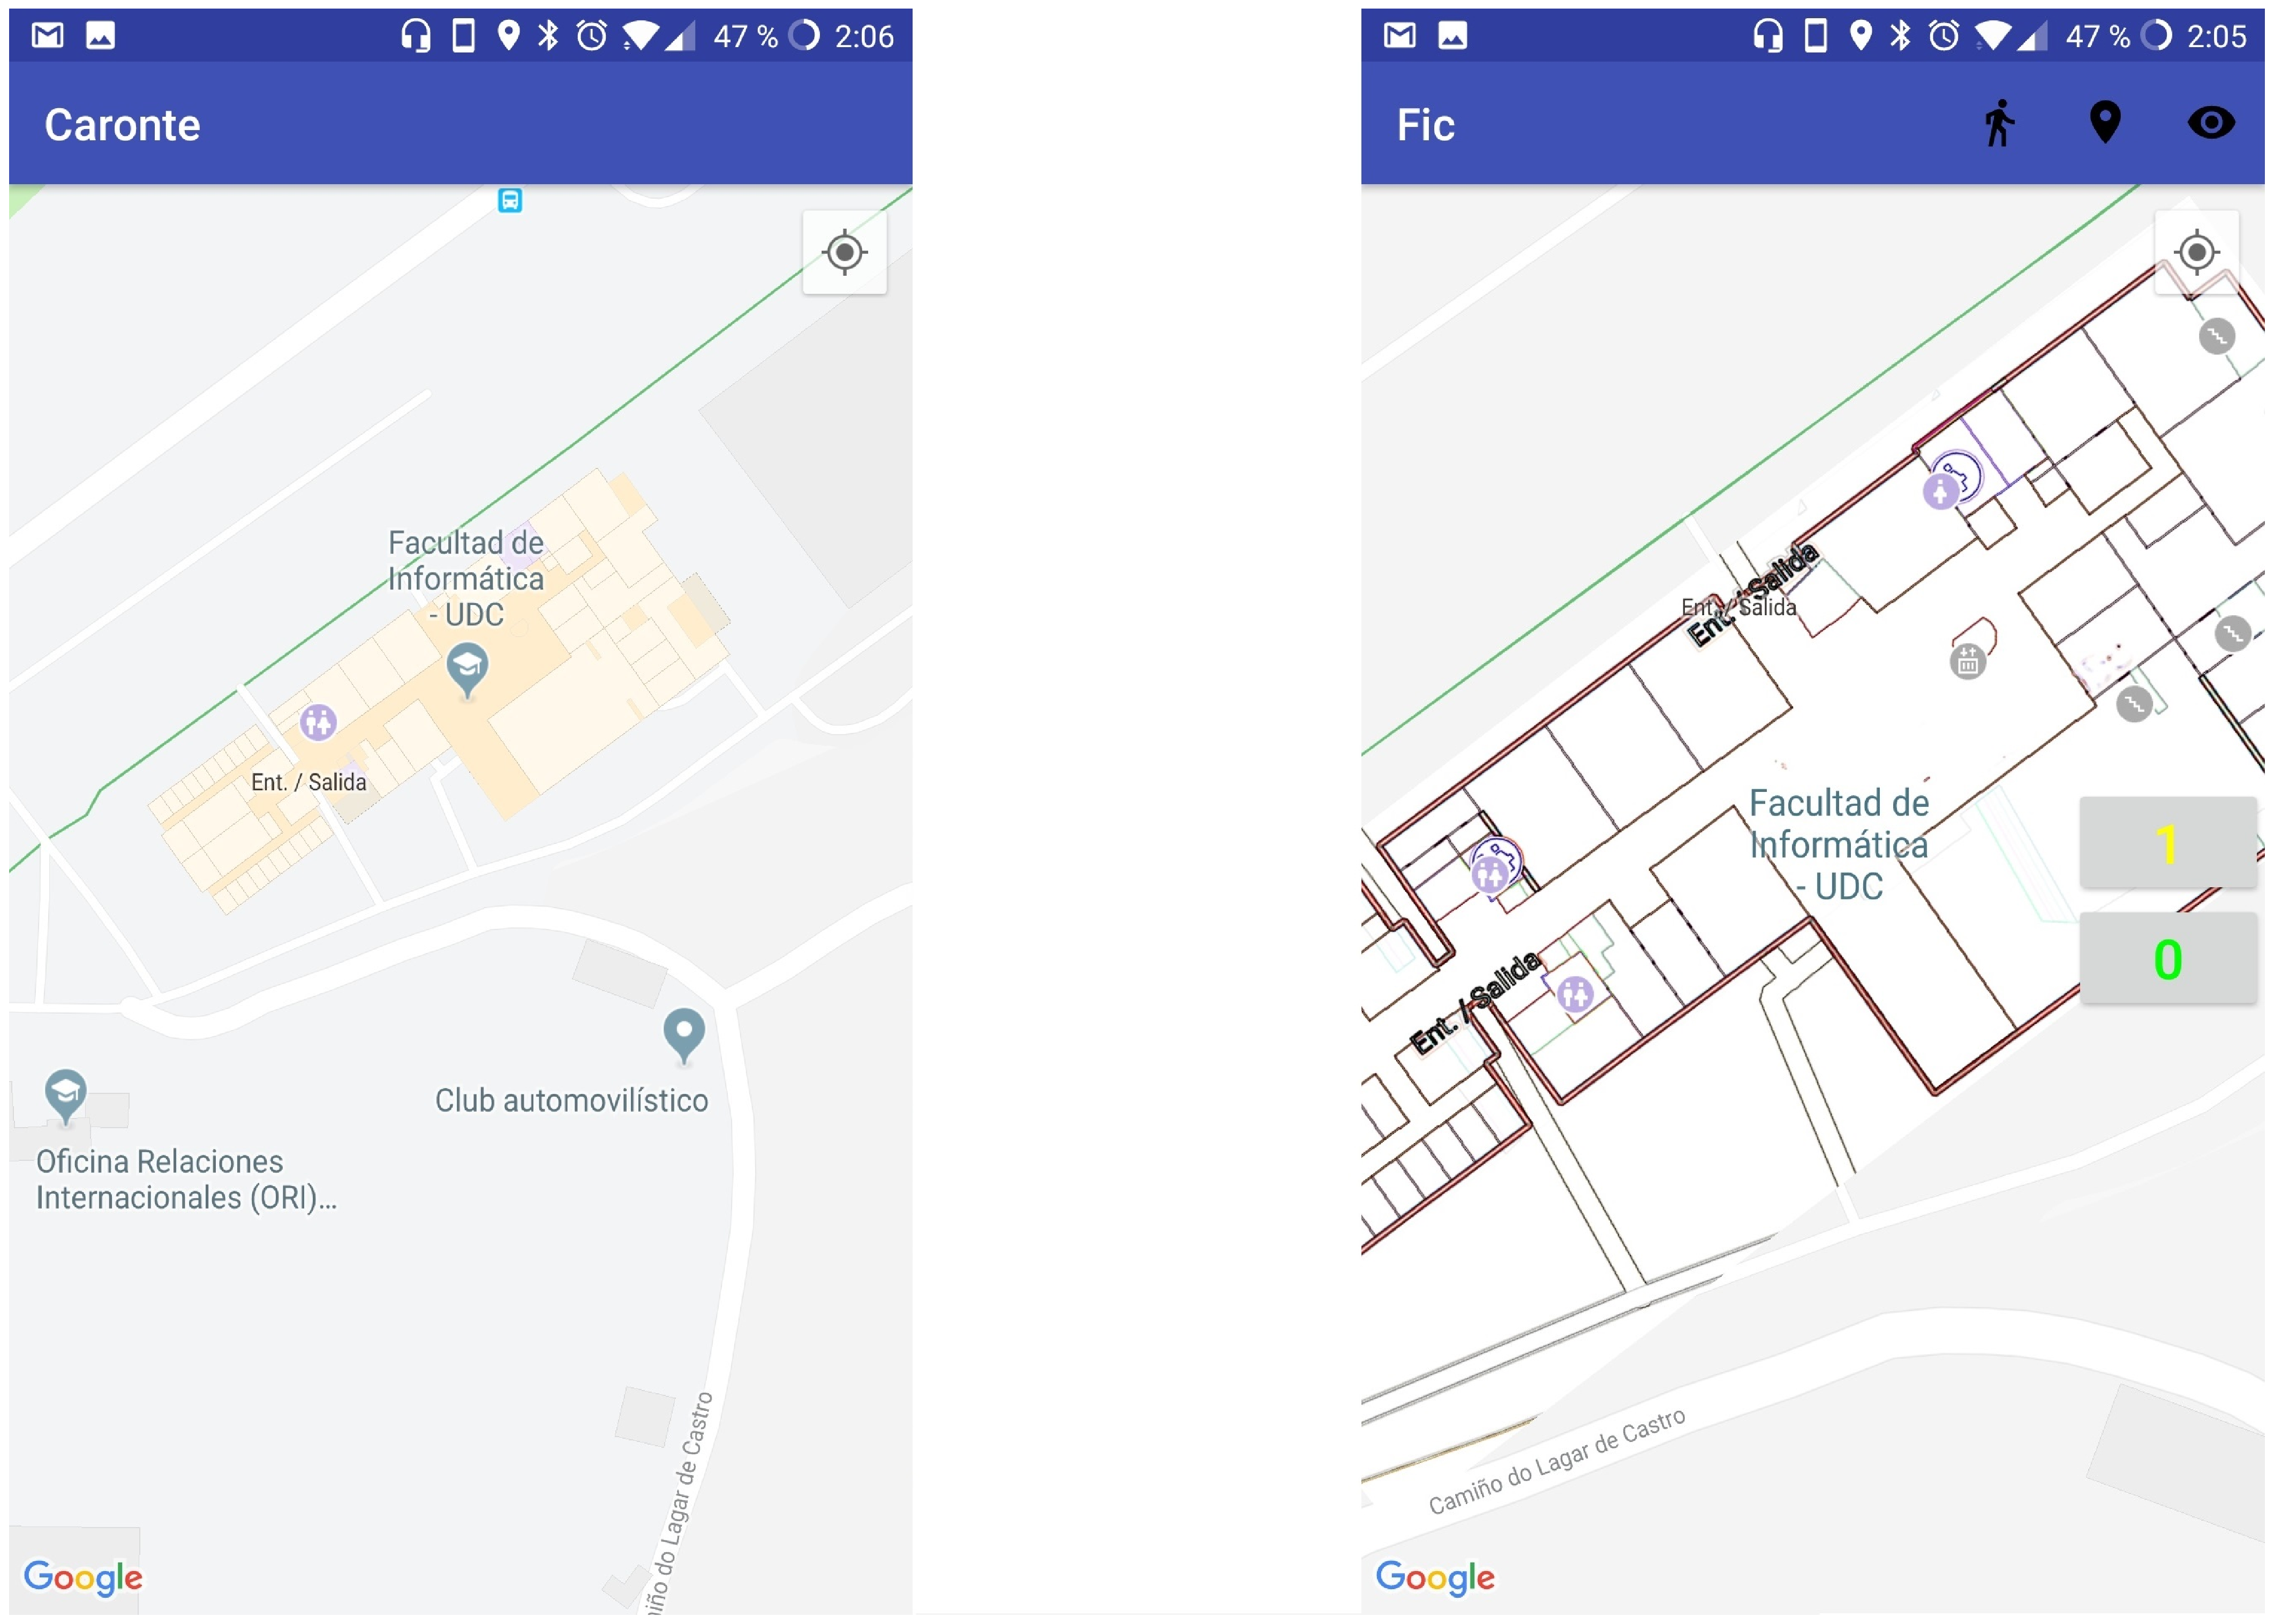
\includegraphics[width=0.5\textwidth]{figures/android/mapaEdificio}
		\caption{Pantalla de mapa sen edificio activo (esquerda), e con edificio activo (dereita).}
		\label{fig:mapaEdificio}
	\end{center}
\end{figure}


\subsection{Mapa}
Esta é a pantalla con máis información dispoñíbel da aplicación e polo tanto, a máis complexa. Na primeira captura que se ve na figura~\ref{fig:mapaEdificio} obsérvase o estado da aplicación cando o usuario non se atopa fisicamente nun edificio configurado, dende ela non poderemos realizar ningunha acción que non sexa buscar un edificio configurado no mapa e pulsar sobre el, accedendo á súa información. Cando se realiza esta acción, aparecerá o mapa do edificio seleccionado, así coma o seu nome e diversos botóns, como se pode ver na segunda captura da figura~\ref{fig:mapaEdificio}.

\begin{figure}[h]
	\begin{center}
		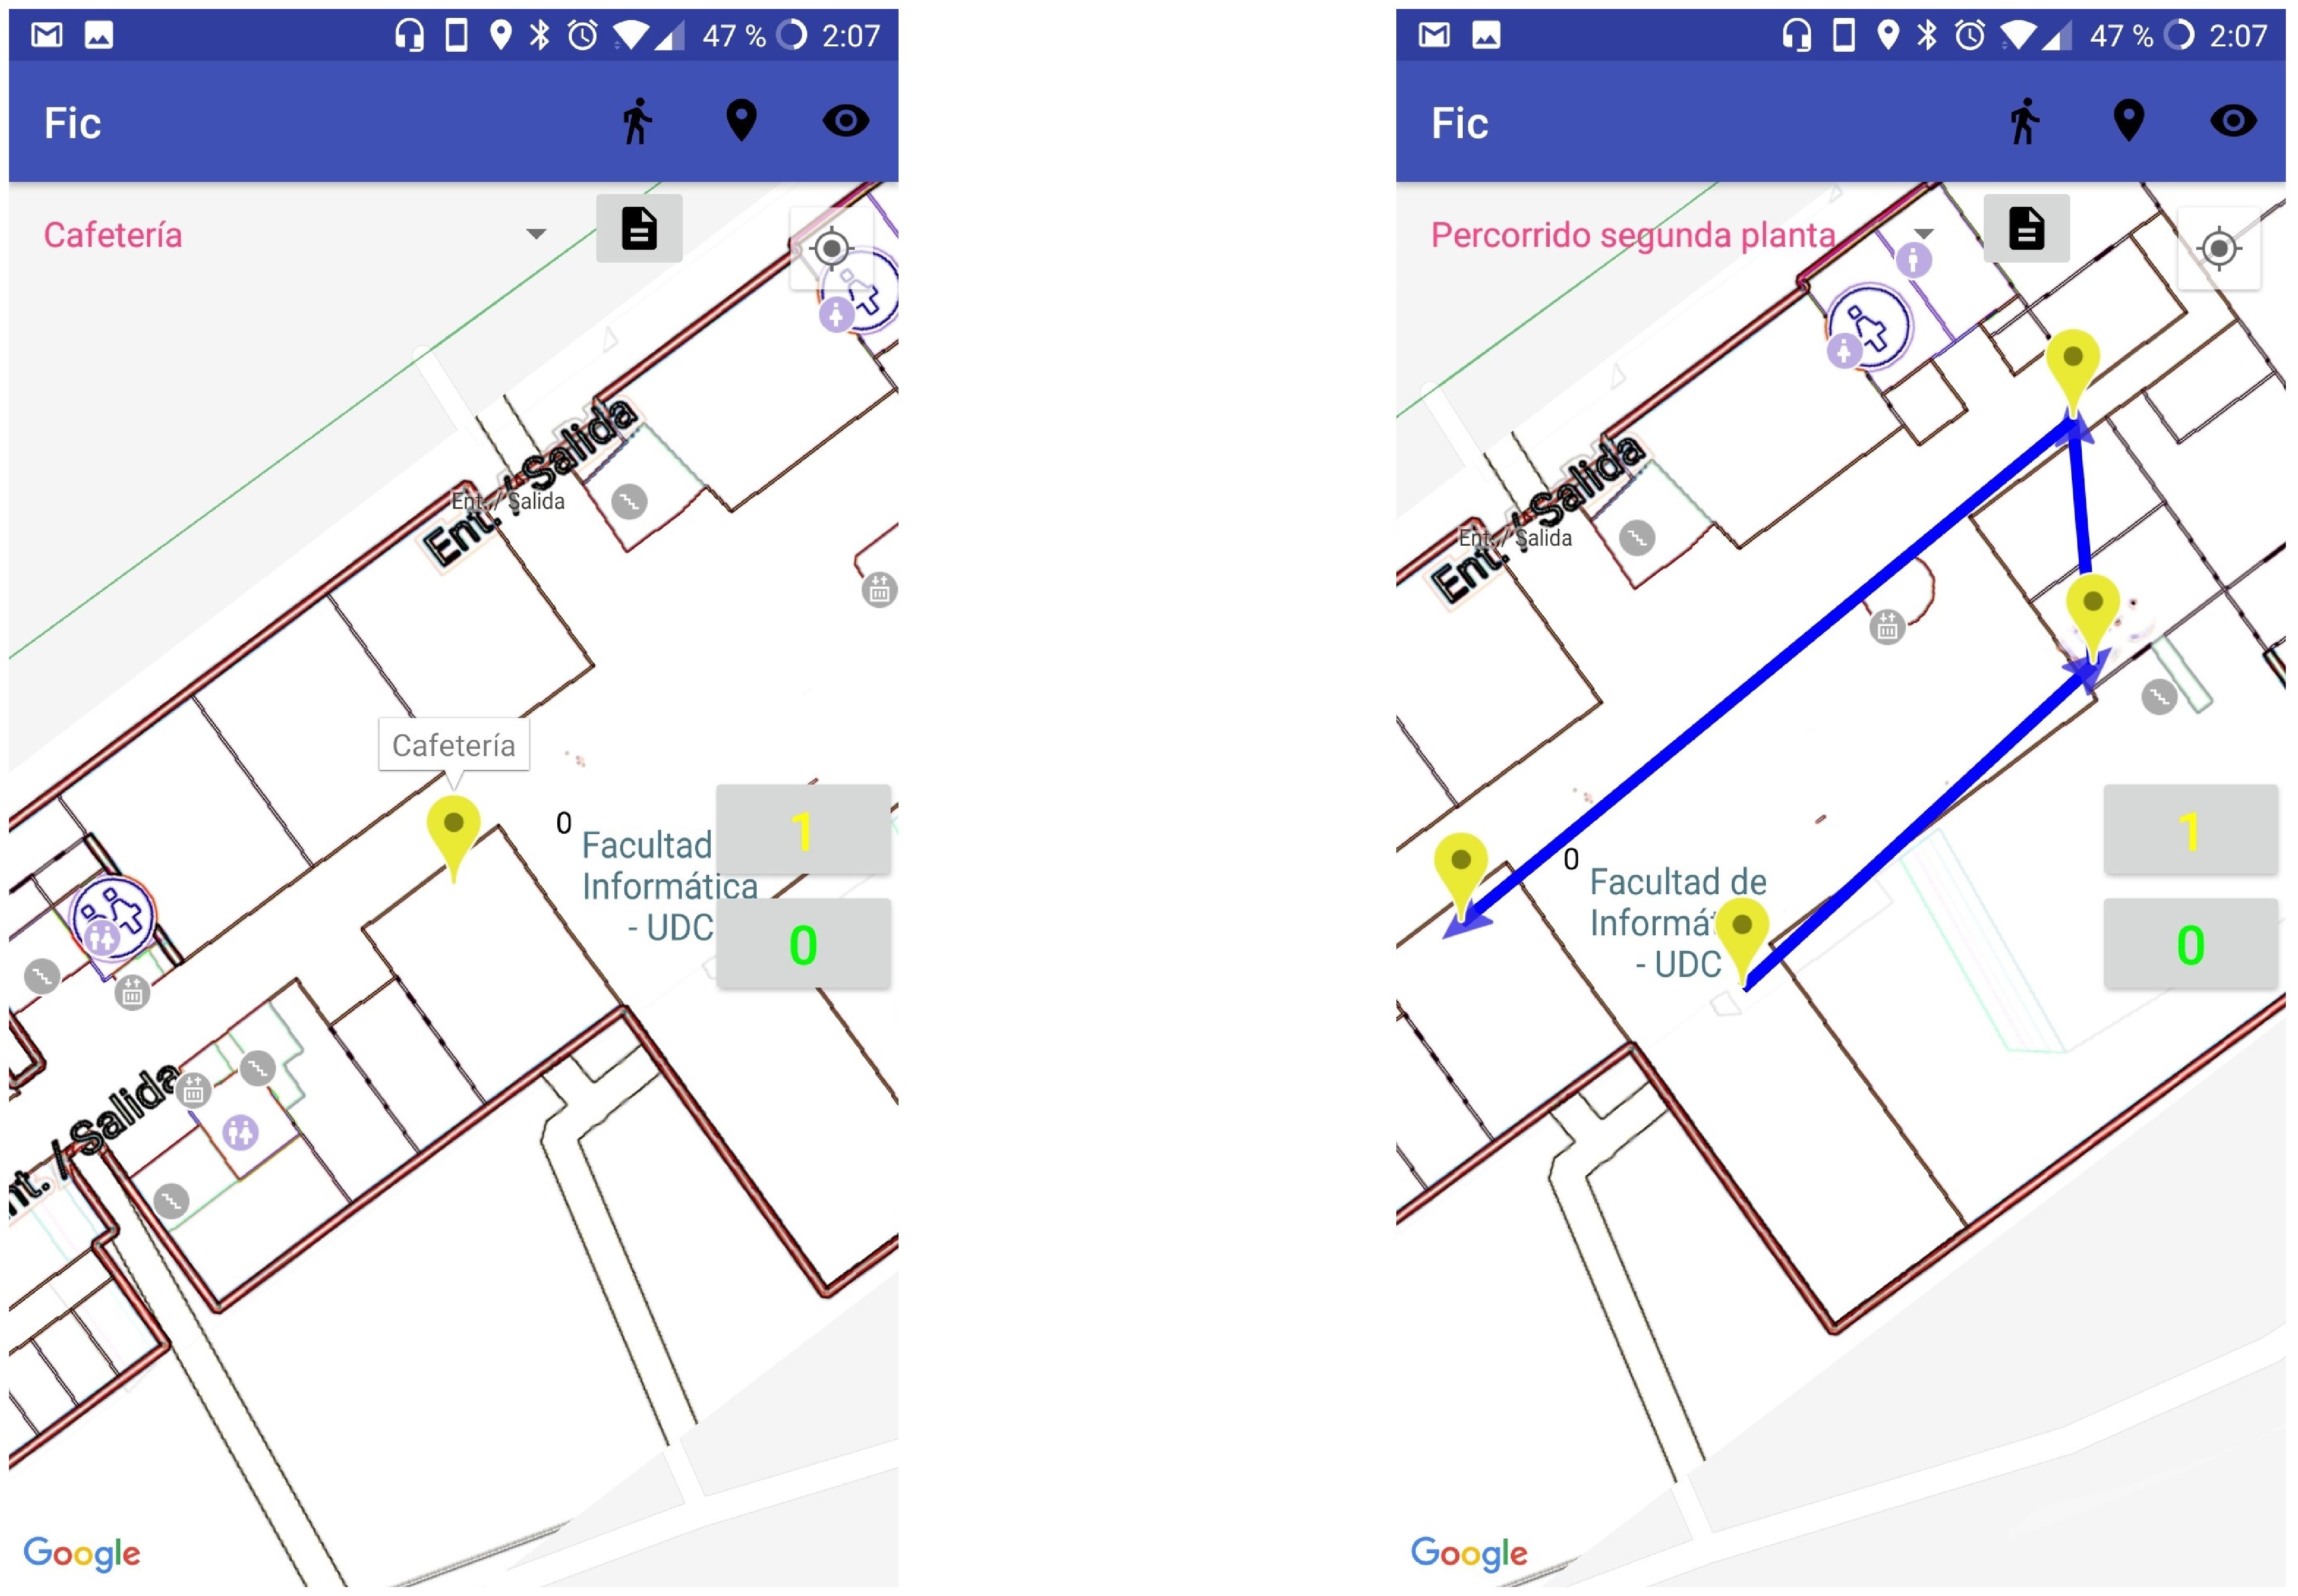
\includegraphics[width=0.5\textwidth]{figures/android/mapaSelector}
		\caption{Pantalla onde se amosan os selectores de POIs (esquerda) e percorridos (dereita).}
		\label{fig:mapaSelector}
	\end{center}
\end{figure}

Os botóns da barra de ferramentas serven para visualizar o spinner cos percorridos, amosar o selector de puntos de interese e mostrar todos os POIs do edificio, respectivamente. Se o edificio ten varios niveis, cárganse os botóns na metade da pantalla que permiten visualizar o mapa desexado. As cores dos números destes botóns coinciden coa cor dos marcadores que indican os puntos de interese dentro do mapa, desta maneira pódense situar máis facilmente. Na figura~\ref{fig:mapaSelector} pódense ver os spinners para os puntos de interese e os percorridos. Cando se ten un deles seleccionado amósase no mapa e permítese acceder aos seus detalles pulsando sobre o botón dereito que aparece á súa dereita.

\begin{figure}[h]
	\begin{center}
		
\includegraphics[width=0.5\textwidth]{figures/android/detallePoiPercorrido}
		\caption{Pantallas de detalle de POIs (esquerda) e percorridos (dereita).}
		\label{fig:detallePoiPercorrido}
	\end{center}
\end{figure}

\subsection{Pantallas de detalle}
Pulsando sobre o botón que aparece á dereita dos spinners accederemos ás pantallas que se poden observar na captura~\ref{fig:detallePoiPercorrido}. Nestas actividades amósase a información gardada sobre os elementos. Na pantalla de detalles para os puntos de interese tamén se poden visualizar imaxes, se dispoñen delas. Habería que pinchar sobre o botón Ver imaxe e seleccionar a imaxe desexada de entre todas as que aparezan no menú contextual.


\section{Manual de usuario da aplicación Caronte para editar contidos}
Todo o indicado na subsección anterior é aplicábel ao xestor de contidos, máis estes usuarios poden realizar máis accións ca un usuario normal. Todos os xestores de contido teñen que autenticarse cunha conta de Google e que esa conta teña permisos sobre o edificio no que se queira engadir contido. A pantalla de inicio é igual que os usuarios normais e tamén o mapa a primeira vista, mais isto cambiará en canto accedamos a un edificio sobre o cal o usuario dispoña de permisos de xestor de contido. A continuación indicaranse cales son as accións que pode realizar e como levalas a cabo.

\begin{figure}[h]
	\begin{center}
		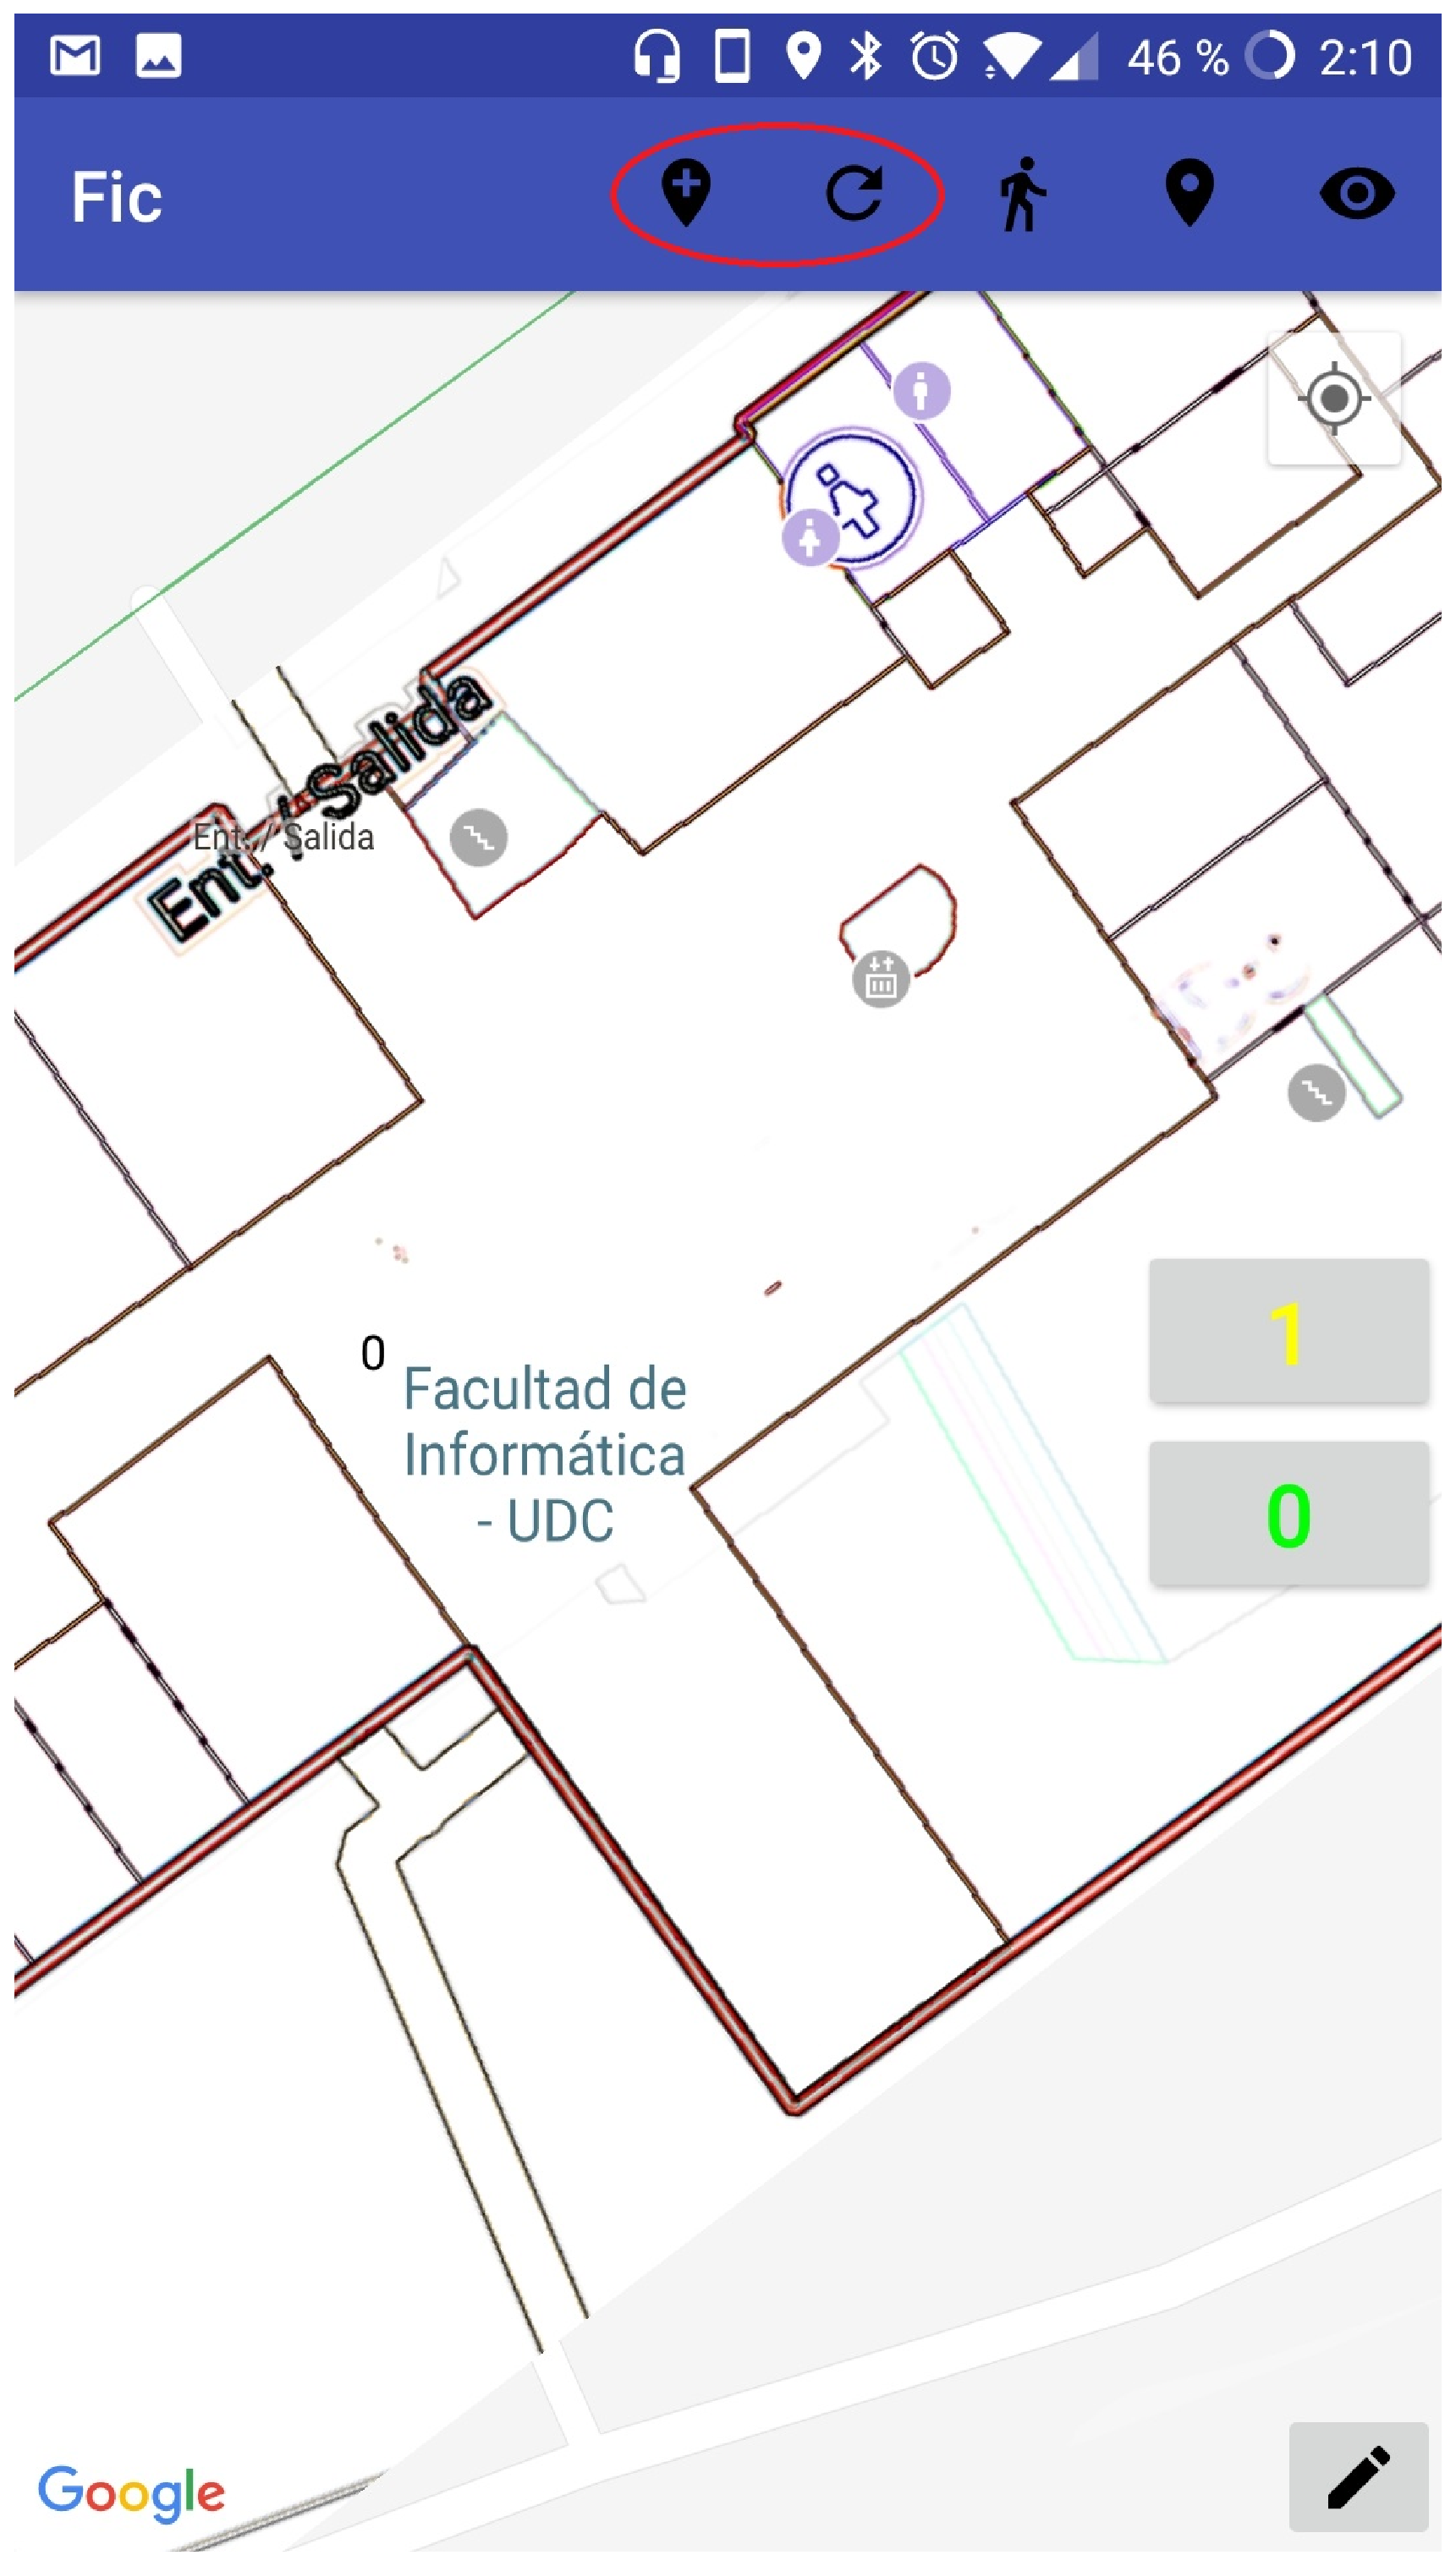
\includegraphics[width=0.25\textwidth]{figures/android/mapaXestorEdicion}
		\caption{Pantalla onde se amosan os botóns de creación de POIs e percorridos.}
		\label{fig:mapaXestorEdicion}
	\end{center}
\end{figure}

\subsection{Activación do modo edición}
O primeiro paso para levar a cabo calquera tipo de acción como xestor de contido é a activación do modo edición dentro dun edificio. Cando se ten seleccionado un edificio sobre o que se ten permisos de xestor de contido, aparecerá na esquina inferior dereita un botón cun debuxo de lapis. Pinchando sobre el, aparecerán dous novos botóns na barra de ferramentas á esquerda dos xa visíbeis. Estes dous novos botóns serven para engadir POIs e crear novos percorridos, respectivamente. Pódense ver estes botóns na figura~\ref{fig:mapaXestorEdicion}.

\begin{figure}[h]
	\begin{center}
		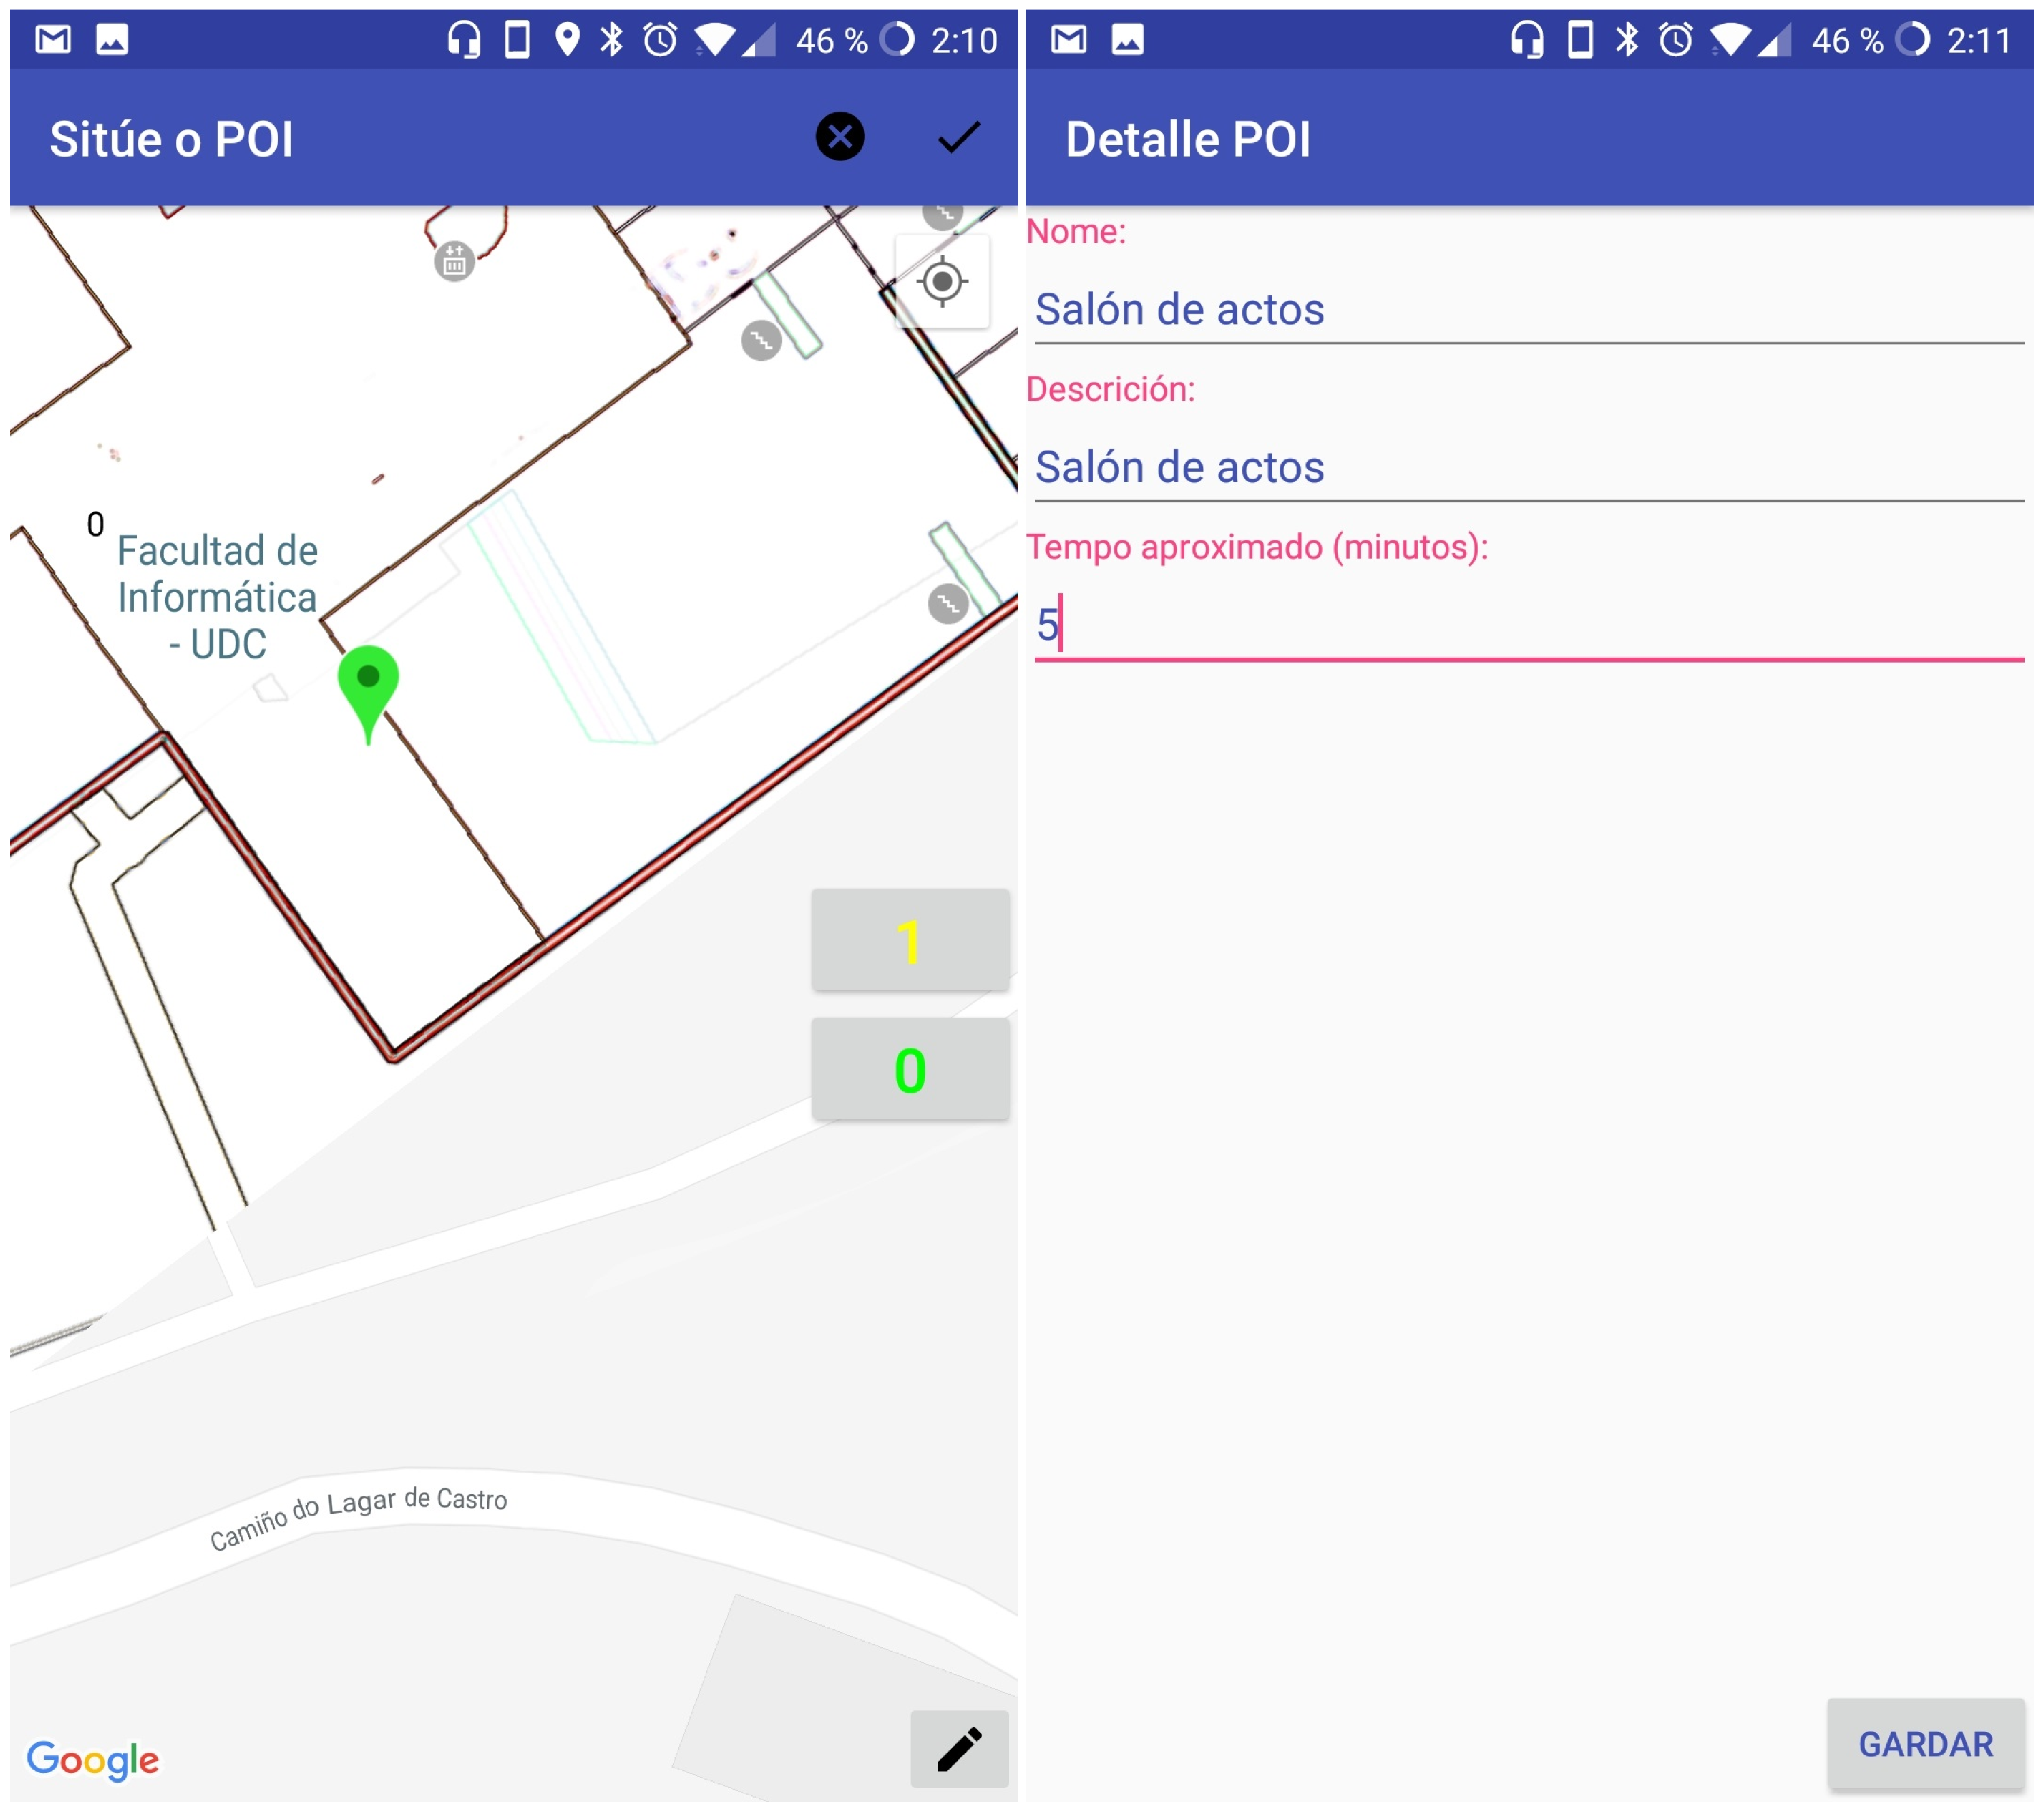
\includegraphics[width=0.5\textwidth]{figures/android/mapaCrearPoi}
		\caption{Capturas do proceso de creación dun POI, localización (esquerda) e inserción de detalles (dereita).}
		\label{fig:mapaCrearPoi}
	\end{center}
\end{figure}

\subsection{Creación de POI}
Pulsando sobre o novo icono que aparece máis á esquerda pódese crear un novo punto de interese. Haberá que situalo no mapa e despois introducir toda a información referente a el, como se pode ver na figura~\ref{fig:mapaCrearPoi}. Se en vez de crear un POI se desexa modificar a súa información poderíase acceder á pantalla de detalle, cambiar os datos desexados e pulsar sobre o botón gardar. Se o que se desexa é eliminalo, débese pulsar sobre o botón Eliminar.

\begin{figure}[h]
	\begin{center}
		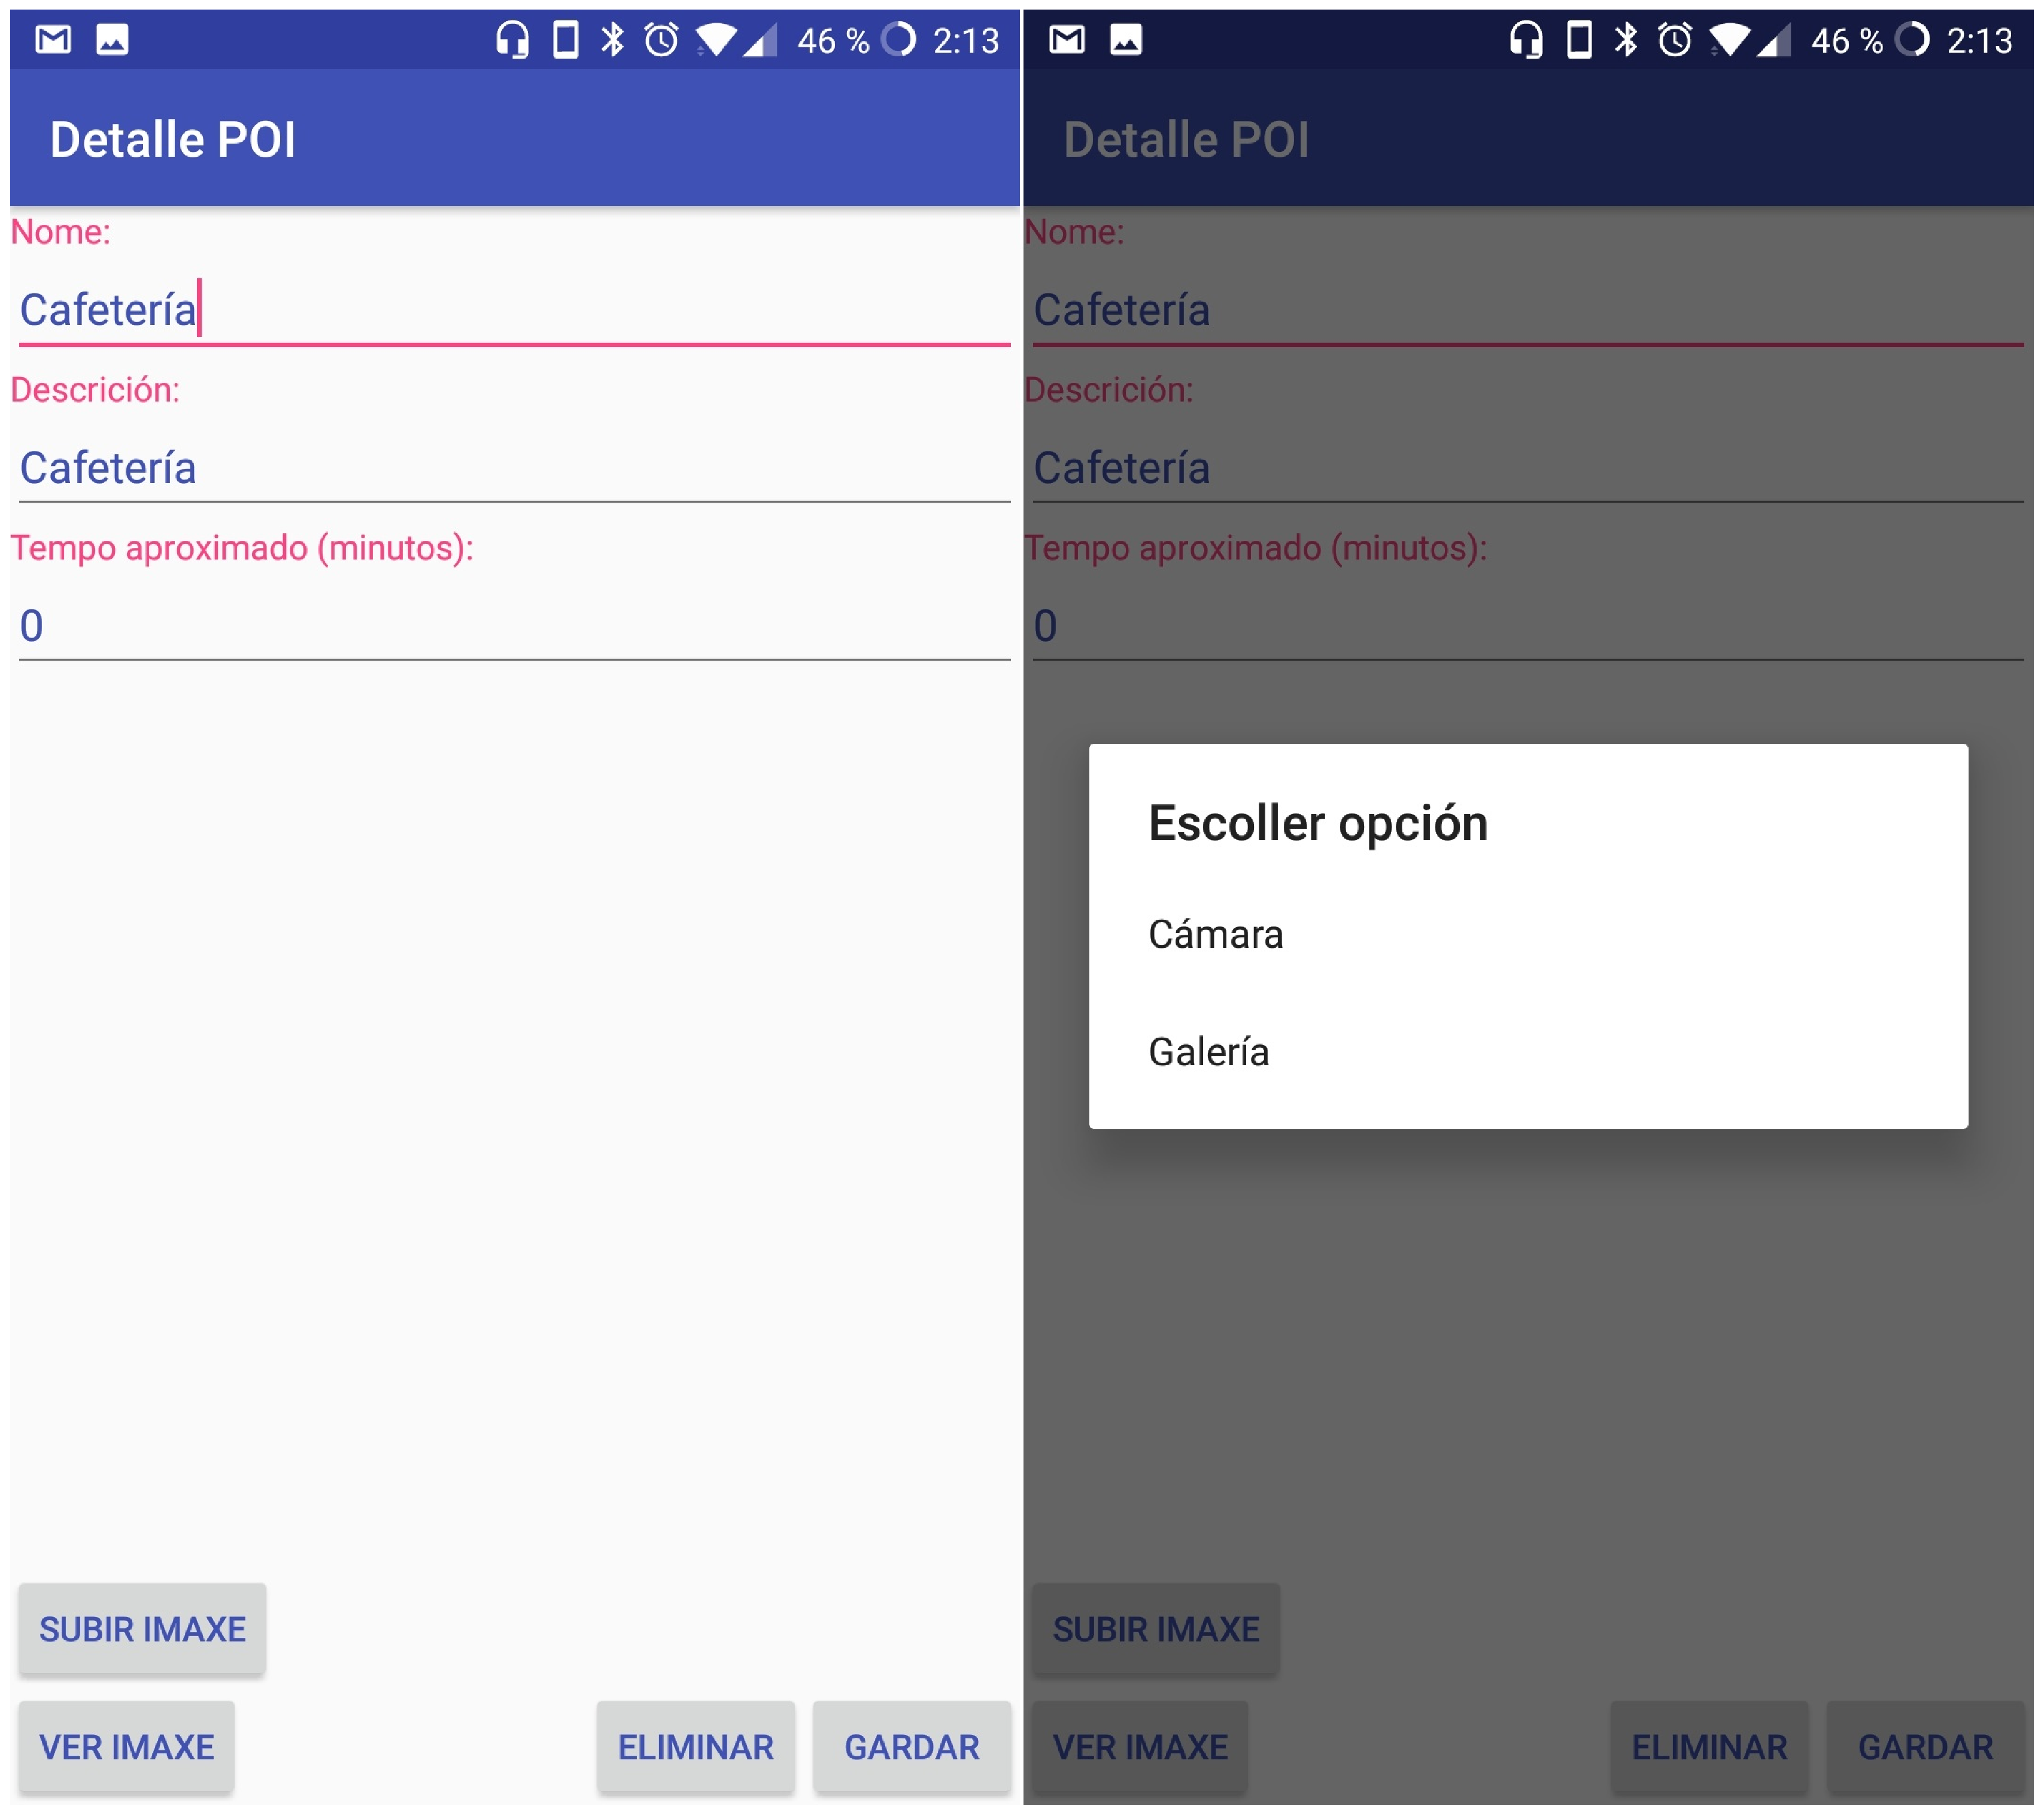
\includegraphics[width=0.5\textwidth]{figures/android/mapaEngadirImaxe}
		\caption{Captura do detalle dun POI ao que se pode engadir imaxes (esquerda) e captura do menú de selección da orixe da imaxe (dereita).}
		\label{fig:mapaEngadirImaxe}
	\end{center}
\end{figure}

\subsection{Engadir imaxe a POI}
Dende a pantalla de detalle dun POI pódense engadir imaxes pulsando sobre o botón de Subir imaxe. A aplicación ofrece dúas opcións para seleccionar a imaxe: sacar unha novo foto coa cámara ou escoller unha imaxe na galería do teléfono móbil. Estas opcións pódense ver na figura~\ref{fig:mapaEngadirImaxe}.

\begin{figure}[h]
	\begin{center}
		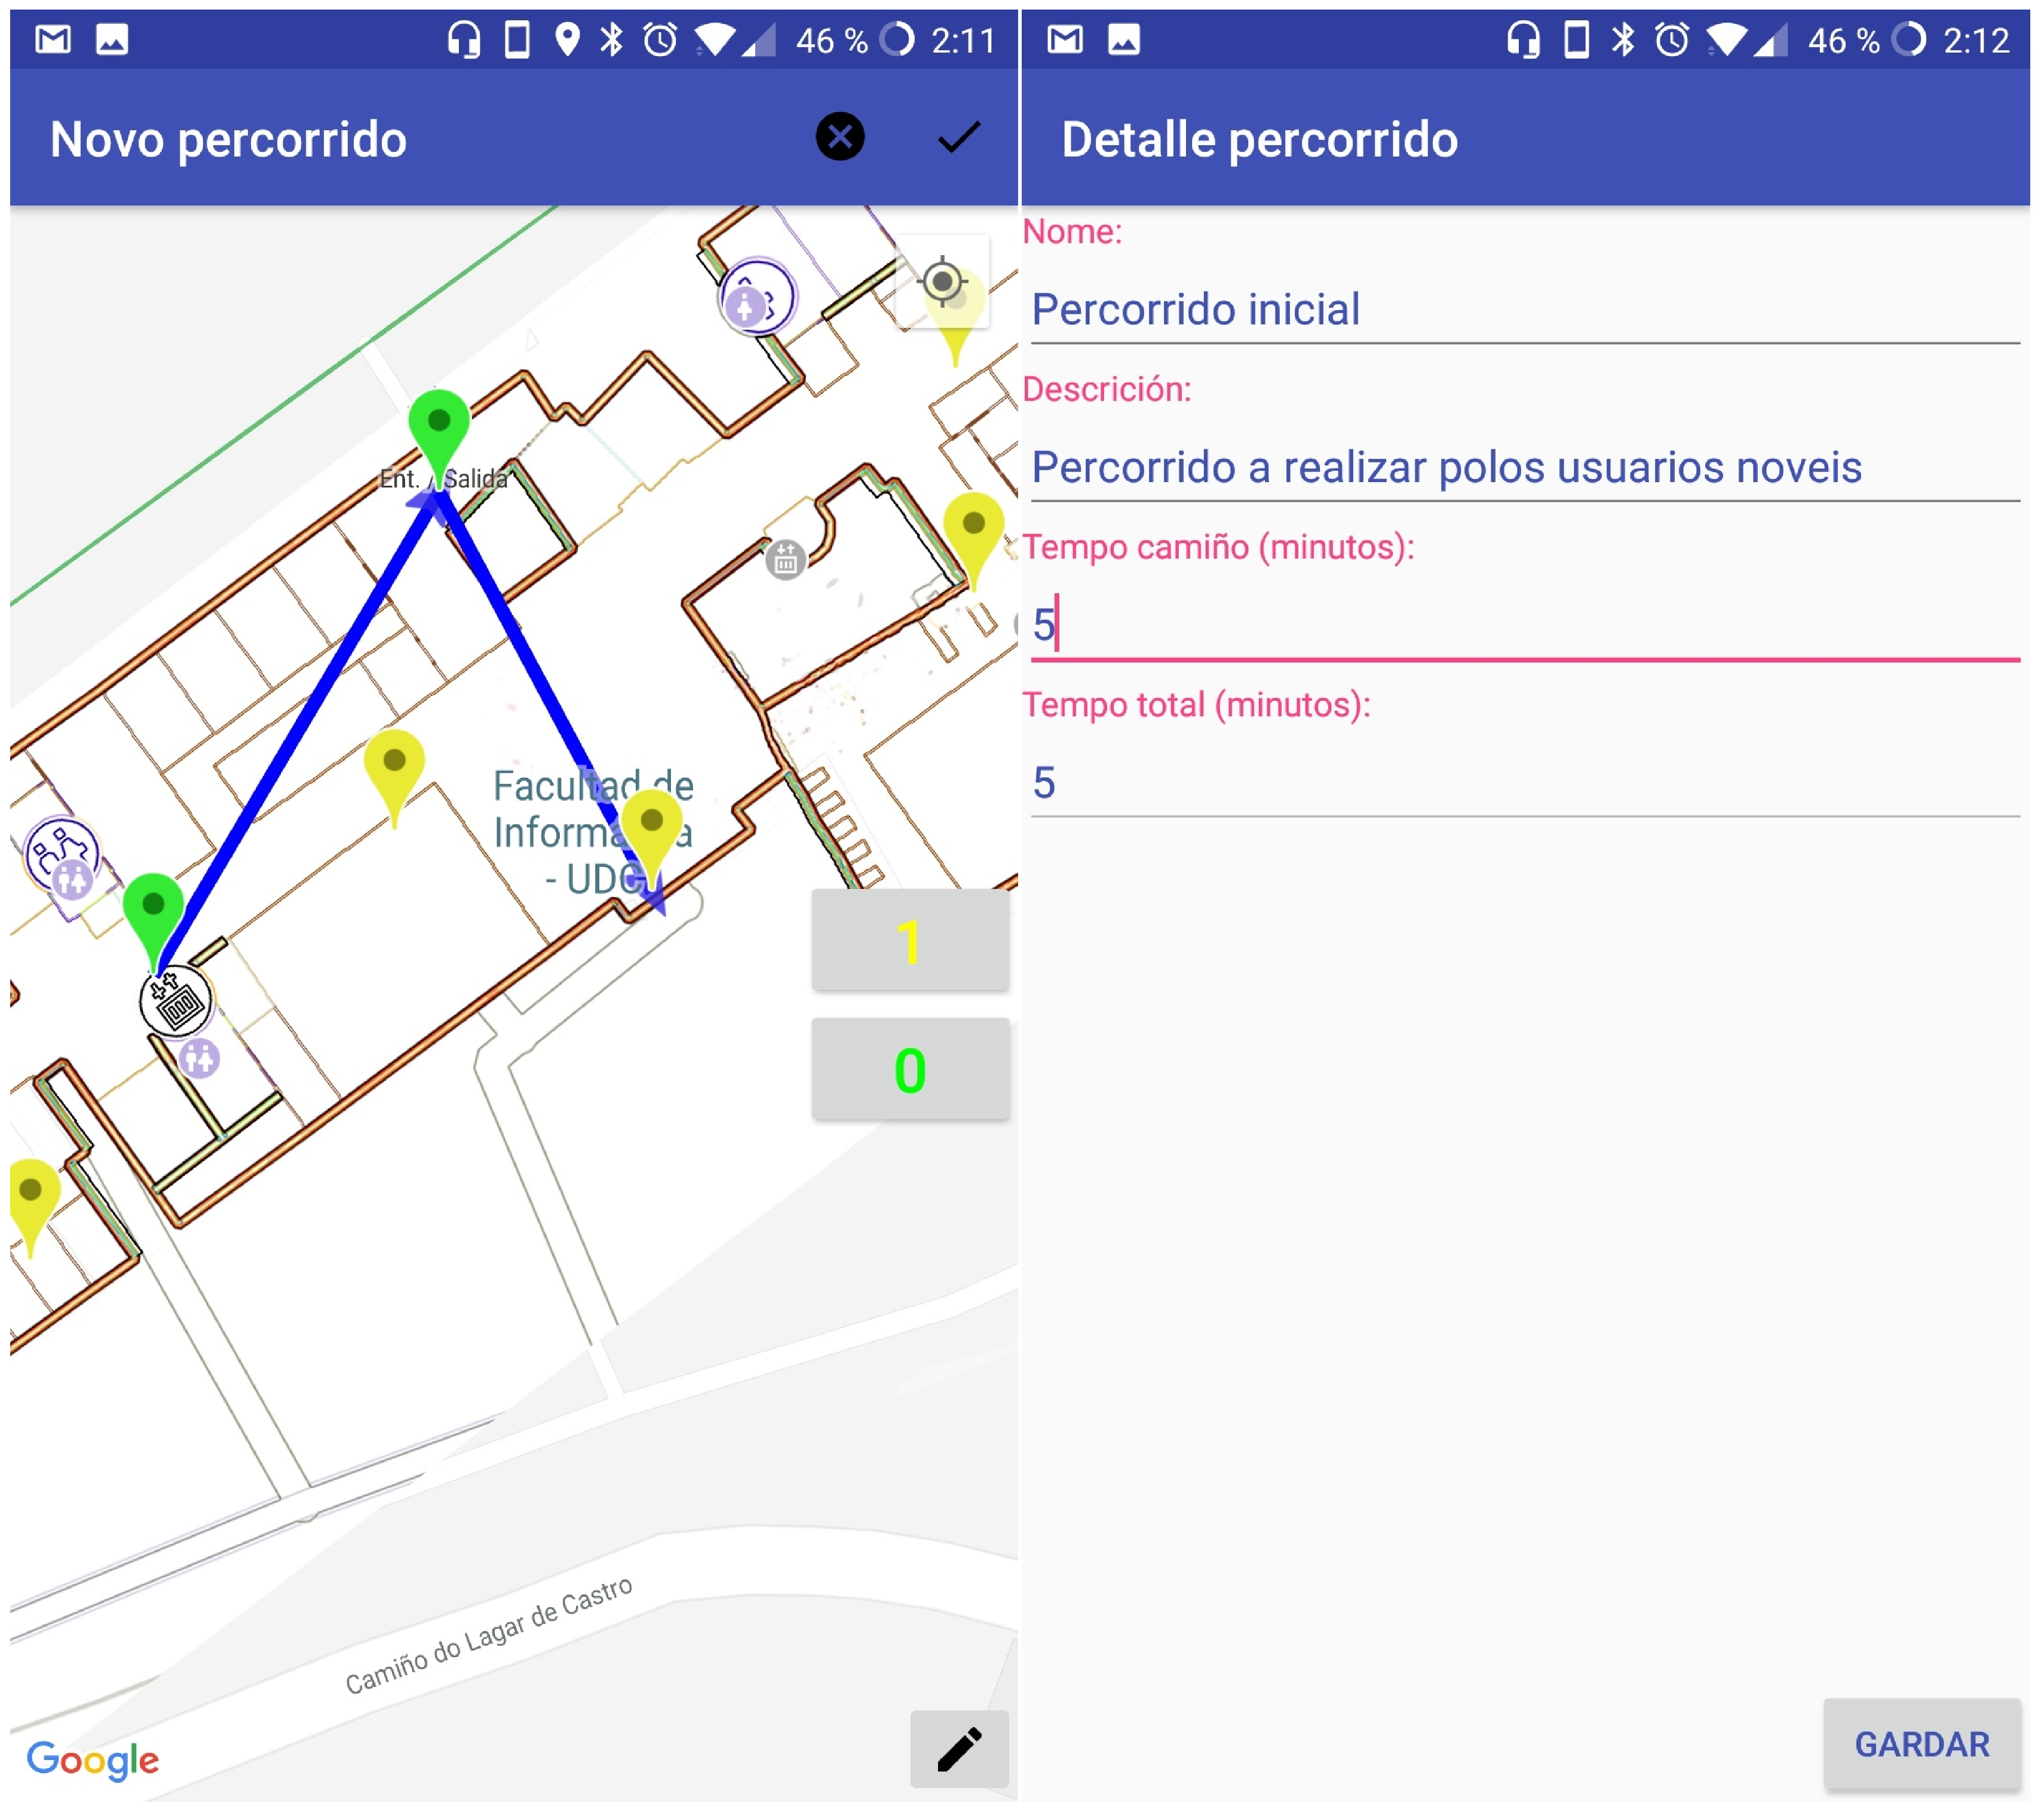
\includegraphics[width=0.5\textwidth]{figures/android/mapaCrearPercorrido}
		\caption{Capturas onde se pode ver a creación dun percorrido: selección de POIs (esquerda) e inserción de datos (dereita).}
		\label{fig:mapaCrearPercorrido}
	\end{center}
\end{figure}

\subsection{Creación de percorrido}
Pulsando sobre a segunda icona de edición pódese crear un percorrido. Débense seleccionar os puntos de interese que se desexan engadir por orde. Unha vez se teñan todos seleccionados, pulsar sobre o tic na parte superior dereita e introducir toda a información referente a el, como se pode ver na figura~\ref{fig:mapaCrearPercorrido}. Se se desexa modificar a información dun percorrido poderíase acceder á pantalla de detalle, cambiar os datos desexados e pulsar sobre o botón gardar. Se o que se desexa é eliminalo, débese pulsar sobre o botón Eliminar.

\begin{figure}[h]
	\begin{center}
		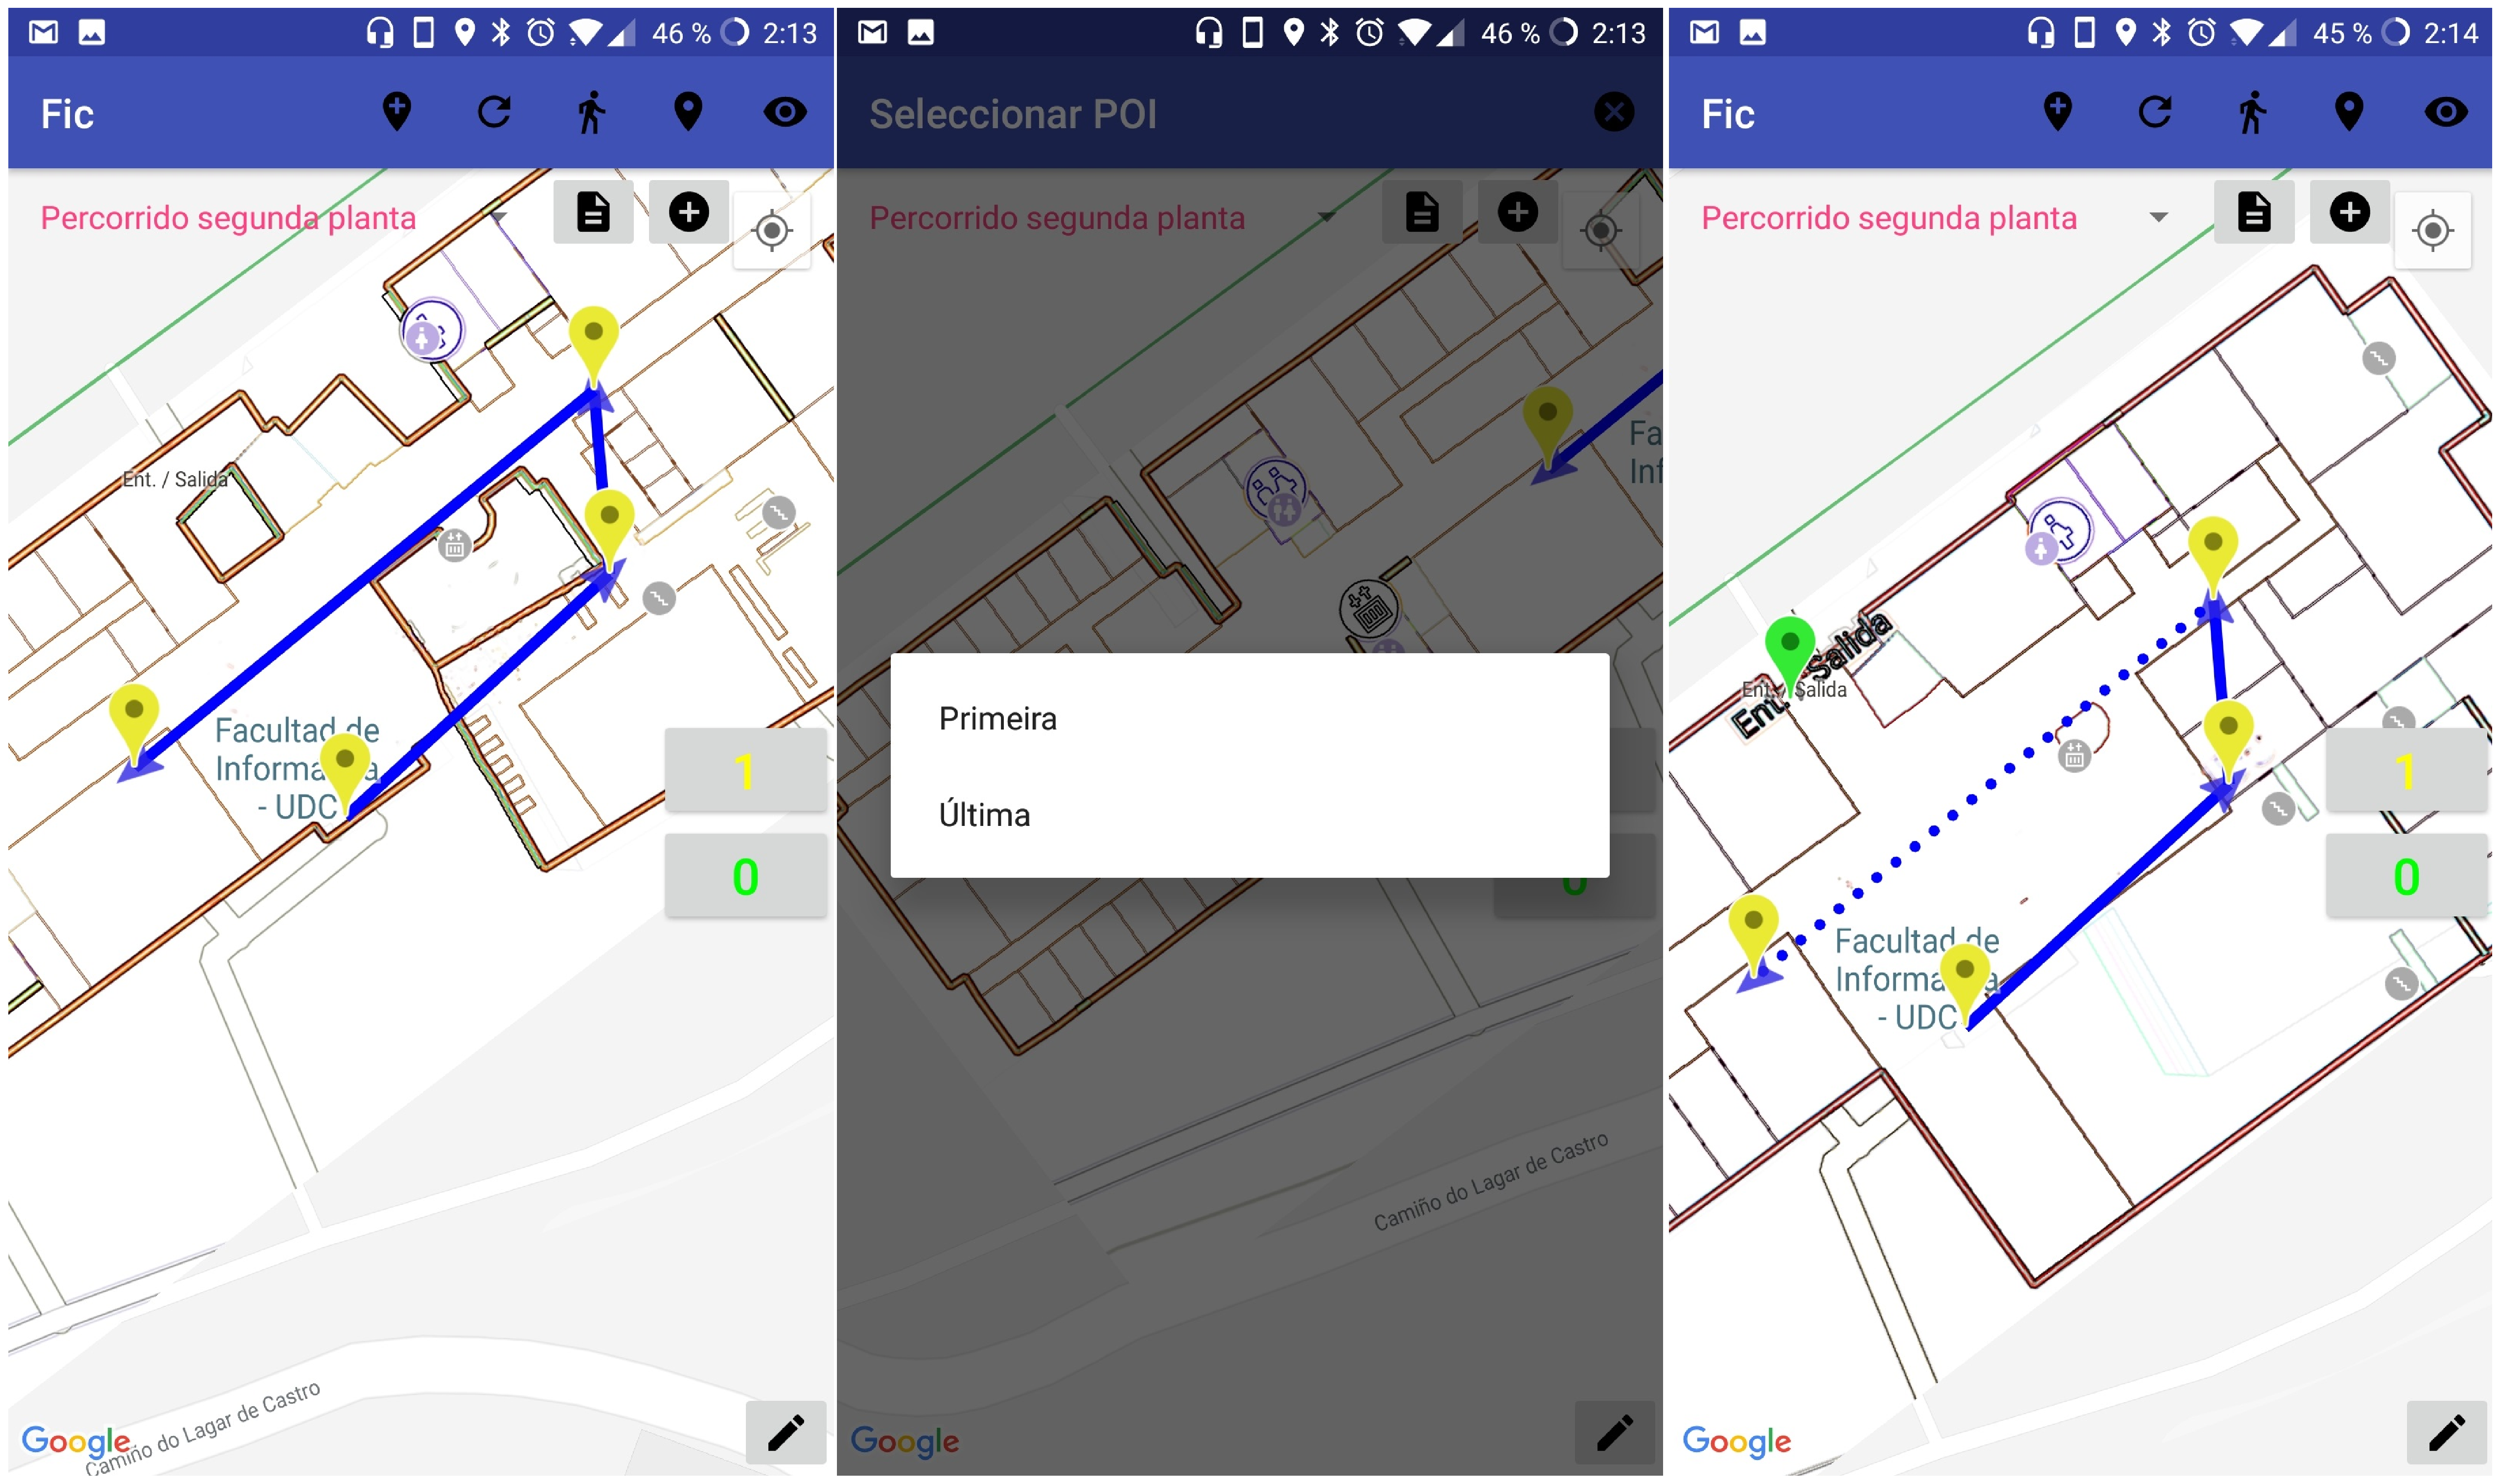
\includegraphics[width=0.7\textwidth]{figures/android/mapaEngadirPoiPercorrido}
		\caption{Capturas onde se pode ver un percorrido modificábel (esquerda), menú contextual despois de seleccionar o POI desexado para escoller a súa posición (centro) e POIs consecutivos entre os que se quere inserir un novo POI (dereita).}
		\label{fig:mapaEngadirPoiPercorrido}
	\end{center}
\end{figure}

\subsection{Engadir ou eliminar POIs nun percorrido xa existente}
Pódense engadir puntos de interese a un percorrido xa existente dende a pantalla principal. Bastaría con seleccionar o percorrido desexado e pulsar sobre o botón cun símbolo ``+'' para que salte a opción de engadir un novo POI ao inicio ou na fin do percorrido. Se se quere inserir un novo POI no medio do percorrido débese seleccionar a liña que une os puntos que se quere separar e a continuación, indicar o novo POI. Estas accións pódense ver na figura~\ref{fig:mapaEngadirPoiPercorrido}.

\begin{figure}[h]
	\begin{center}
		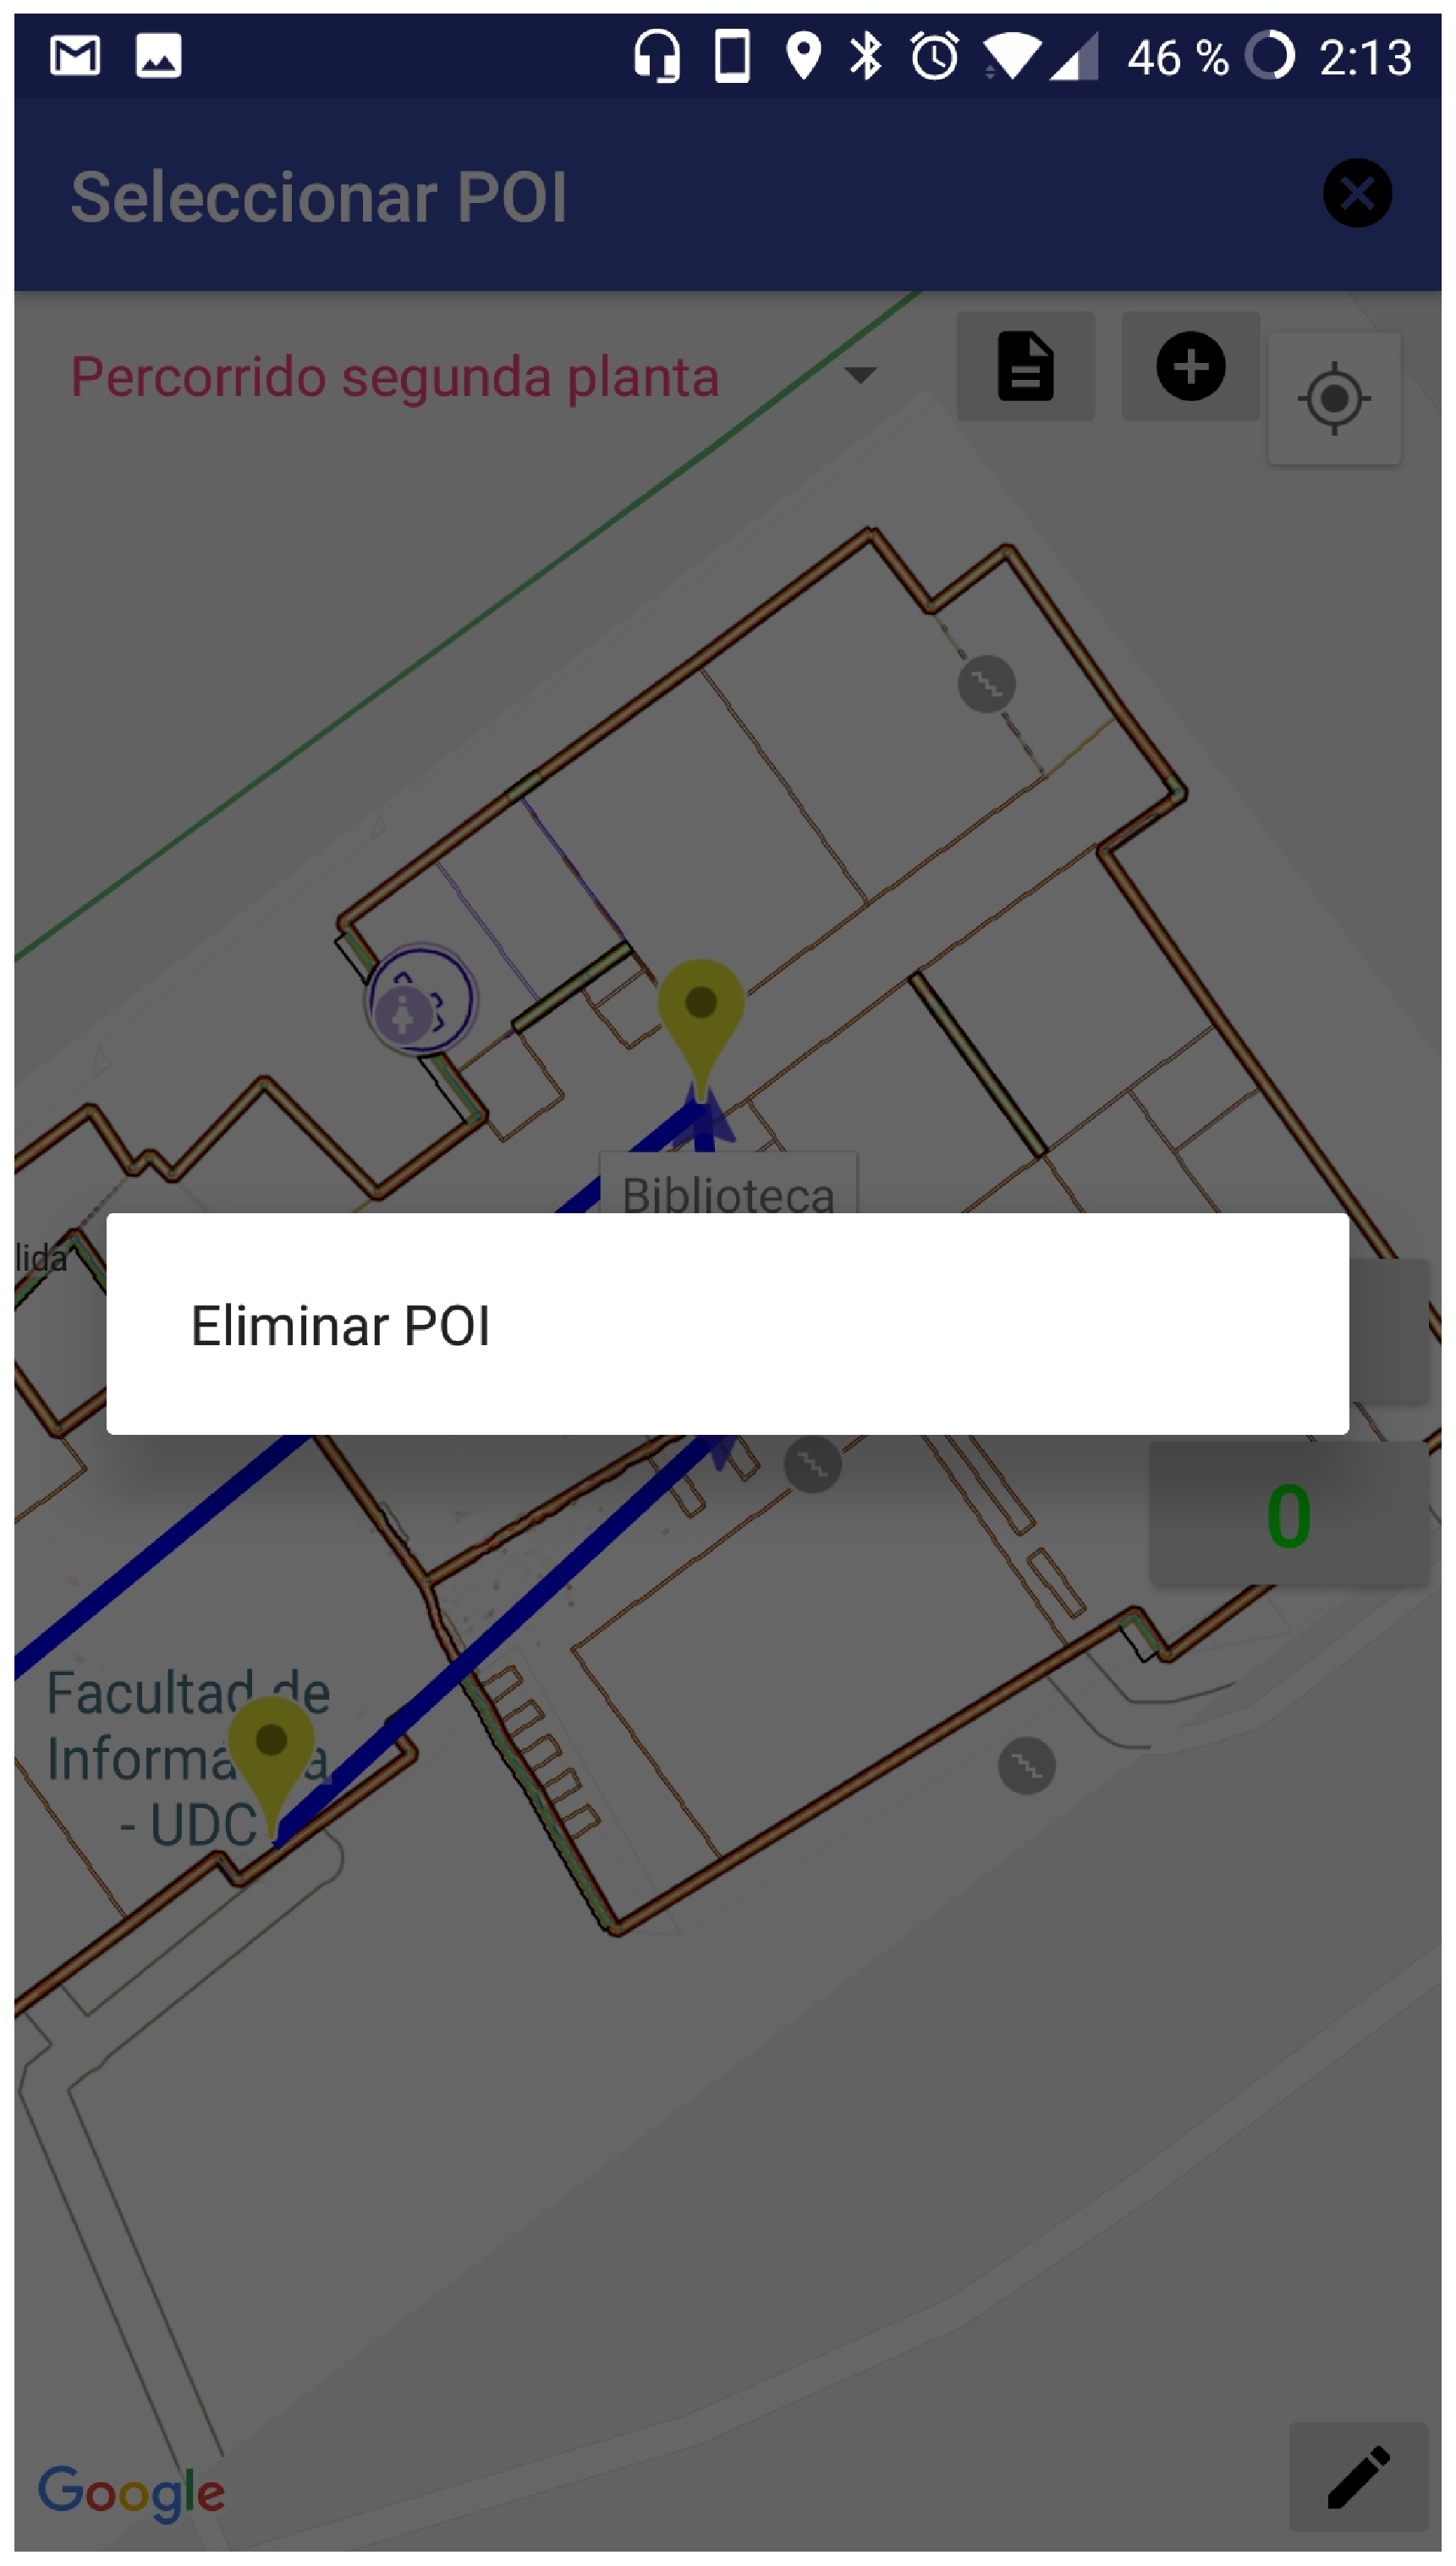
\includegraphics[width=0.25\textwidth]{figures/android/mapaEliminarPoiPercorrido}
		\caption{Captura onde se pode ver a eliminación dun POI dun percorrido.}
		\label{fig:mapaEliminarPoiPercorrido}
	\end{center}
\end{figure}

Se pola contra o que se quere é quitar un punto de interese dun percorrido, debemos pinchar sobre o marcador do punto desexado e seleccionar a opción Eliminar como se pode ver na figura~\ref{fig:mapaEliminarPoiPercorrido}.

